\cotefile{71}

\scanpage{7}

\diagram{\resizebox{\linewidth}{!}{\begin{tikzpicture}[x=.012cm,y=-.012cm,every node/.style={inner sep=1pt}]
\node[anchor=north west] at (30,60) {\begin{tikzcd}[ampersand replacement=\&,row sep=1pt,column sep=2pt]
\& e\in E\\
\& \cup\\
M(e)\ \subset \& E_0=M(E) \arrow[ddd,"\varphi"]\\[-.4ex]
\shortparallel \&\\[-.4ex]
M(E_e) \&\\
\& I\quad\text{ordonné}
\end{tikzcd}};
\node[anchor=north west] at (575,77) {$\displaystyle
\left\{\begin{aligned}
|E|&=X\supset|E_e|\\
X_i&=\bigcup_{\varphi(M(e))\leq i}|E_e|
\end{aligned}\right.$};
\node[anchor=north west] at (1258,83) {$E_e=\{x\in E\mid x\leq e\}$};
\draw (1135,253) .. controls (1300,224) and (1515,207) .. (1629,197);
\draw (1117,298) .. controls (1101,345) and (1078,578) .. (1076,643);
\node[anchor=north west] at (1124,323) {\begin{tikzcd}[ampersand replacement=\&,row sep=2pt]
e_0\in E_0\arrow[d,mapsto]\\
X_{e_0}=\displaystyle\bigcup_{M(e)\leq e_0}|E_e|
\end{tikzcd}};
\node[anchor=north west] at (354,509) {$
(i_0>\mathord{-}\mathord{-}>i_k)=
\underset{\substack{\cap\\I}}d\in\operatorname{Drap}(I)$};
% Faint three-armed trace immediately above the first boundary symbol.
\draw[gray!60,very thin] (1211,612)--(1286,646)--(1359,599) (1286,646)--(1308,718);
\node[anchor=west] at (342,766) {$\Sigma_d(\mathcal X)$};
\node[anchor=west] at (737,753) {$\Sigma_{\{i\}}(X)=\Sigma(X_i,\partial X_i)$};
\node[anchor=north west] at (428,865) {\begin{tikzcd}[ampersand replacement=\&,column sep=8pt,row sep=16pt,cells={nodes={inner sep=1pt}}]
\Sigma_{\{i_0,-,\unsure{i_{k_{i-1}}|i_{ki-1}}\}}(\mathcal X)
  \arrow[r,phantom,"\supset" description]\arrow[d]
\& \partial\Sigma_{\{i_0,-i_{k-1}\}}\arrow[r,phantom,"\supset" description]\arrow[dd,dash]
\& \deleted{\unsure{\partial}}\Delta_{i_0-i_k}(\mathcal X)\arrow[r,phantom,"\supset" description]\arrow[dd]
\& \partial\Delta_{i_0-i_k}\arrow[dd]\\
\Sigma_{i_{k-1}}(X)\deleted{\unsure{i_k}}\arrow[d] \& \& \&\\
X_{i_{k-1}}\arrow[r,phantom,"\supset" description] \&
\partial X_{i_{k-1}}\arrow[r,phantom,"\supset" description] \&
X_{i_k}\arrow[r,phantom,"\supset" description] \& \partial X_{i_k}
\end{tikzcd}};
\node[anchor=north west] at (323,1410) {$\Sigma_{\{i_0,-i_k\}}(\mathcal X)=
\Sigma\bigl(\Delta_{i_0-i_k},\partial\Delta_{i_0-i_k}\bigr)$};
\node[anchor=north west] at (113,1634) {$d'\subsetneq d$};
\node[anchor=north west] at (371,1518) {\begin{tikzcd}[ampersand replacement=\&,row sep=12pt]
{} \arrow[d]\\ \Sigma_{d'}(\mathcal X)
\end{tikzcd}};
\draw (249,1911) .. controls (283,1800) and (340,1784) .. (454,1762)
 .. controls (594,1732) and (676,1748) .. (700,1677)
 .. controls (721,1620) and (751,1559) .. (775,1539);
\node[anchor=north west] at (124,1820) {\begin{tikzcd}[ampersand replacement=\&,row sep=23pt]
\Sigma_d\arrow[d]\\ \Sigma_{\widetilde d'}\arrow[d]\\ \Sigma_{d'}
\end{tikzcd}};
\node[anchor=north west] at (364,1529) {\begin{tikzcd}[ampersand replacement=\&,row sep=9pt,column sep=38pt]
\& \partial X_{\unsure{i_{j_k}|j_{i_k}|i_k}}\\
\& X_{\unsure{j_k|i_k}}\arrow[u,phantom,"\rotatebox{90}{$\supset$}" description]\arrow[d,dash]\\
\Sigma_{d\smallsetminus\{i_k\}}\arrow[r]\arrow[d] \&
X_{i_{k-1}}\arrow[d,hook,dash]\\
\Sigma_{d'\smallsetminus\{i_k\}\deleted{\unsure{\cap d'}}}\arrow[r] \&
X_{i_\alpha}\\
\deleted{\Sigma_{d'}}\arrow[u,phantom,"\deleted{\unsure{\downarrow|\updownarrow}}" description] \&
\end{tikzcd}};
\node[anchor=west] at (1183,1791) {$\pi_0(\Sigma_d)=D(d)$};
% Continuous fine oblique through the working, and shorter counterstroke at the foot.
\draw[very thin] (580,114) .. controls (736,658) and (983,1471) .. (1238,2192);
\draw (1009,2162) .. controls (1038,2033) and (1119,1831) .. (1159,1723);
\end{tikzpicture}}}
% archive sheet number: 6

\scanpage{8}

5) Soit $K$ un fermé de l'espace $X$, $(\deleted{\unsure{K}}U{}^{\deleted{\unsure{q|\prime}}}_i{}_{\deleted{\unsure{k|K}}})_{i\in I}$ une famille d'ouverts relatifs de $K$, mutue\uline{llement disj}oints, tels que $\dot K\subset\bigcup_i U_i{}_{\deleted{k}}$. \inserted{Soit $B_i=\dot K\cap U_i$, de sorte que $\dot K=\coprod_i B_i$.} \deleted{Supposons q} Pour $\forall i$, soit $C_i=\overline U_i{}_{\deleted{k}}\smallsetminus U_i{}_{\deleted{k}}$ la frontière relative de $U_i{}_{\deleted{k}}$ dans $K$, supposons que $C_i\subset\bigl(K-\overline U_i{}_{\deleted{k}}\bigr)^{\! -}$ (cf\ldots). Posons $\deleted{\unsure{X}}\deleted{\unsure{U_i}}X_i=X\smallsetminus U'_i$. Alors
\[
\left\{\begin{aligned}
&X_i\ \text{est loc fermé}\\
&\operatorname{Int}X_i=X\smallsetminus\overline{U'_i}=X_i\smallsetminus C_i\\
&\overline X_i=X_i\cup \dot B'_i\qquad(B'_i=\dot K\smallsetminus B_i)
\end{aligned}\right.
\]
% slanted
\margin{\deleted{i.e.\ $C_i$}}

$\operatorname{Int}X_i$ et \uline{$U_i\smallsetminus C_i$} sont \deleted{deux} ouverts de $X$ dont chacun est le complémentaire de l'adhérence de l'autre.

Soit $W=X\smallsetminus K$, \deleted{\unsure{semble}} donc \inserted{$\dot W={}$} $\overline W\cap K=\dot K=\coprod B_i$, l'inclusion $W\subset X_i$ est une imm ouvert et $\dot W\cap X_i=\dot K\cap X_i=B_i$; \deleted{$\unsure{X_i}$} i.e \deleted{\unsure{un}}\deleted{\unsure{l'on}} l'adh. de $W$ dans $X_i$ est $W\cup B_i$, donc la \deleted{bord}\inserted{frontière} de $W$ dans $X_i$ est $B_i$. On a
\[
X_i=(\overline W\cap X_i=W\cup B_i)\amalg_{B_i}\overline U_i
\]

% margin note written sideways (upside down)
\margin{\deleted{Monsieur le \unsure{A|P|D}}}

Alors \unsure{le|la} somme amalgamée de tous les \unsure{$X_i$} sur $W$ est un espace
% Last line meets the lower edge of the scan.
% archive sheet number: 7

\scanpage{9}
% The printed face is read after a half turn.
% letterhead
\figure{
\begin{tikzpicture}[x=.23cm,y=.23cm]
\fill (0,.18) circle (.18);
\fill (-.05,1.13)--(-.23,1.03)--(-.23,.56)--(-.49,.81)--(-.64,.71)--(-.31,.37)
 .. controls (-.20,.28) and (-.05,.34) .. (-.05,.48)--cycle;
\fill (.05,1.13)--(.23,1.03)--(.23,.56)--(.49,.81)--(.64,.71)--(.31,.37)
 .. controls (.20,.28) and (.05,.34) .. (.05,.48)--cycle;
\fill (-.69,.67)--(-.76,.49)--(-.50,.24)--(-.88,.24)--(-.93,.04)--(-.39,.04)
 .. controls (-.20,.05) and (-.17,.19) .. (-.28,.30)--cycle;
\fill (.69,.67)--(.76,.49)--(.50,.24)--(.88,.24)--(.93,.04)--(.39,.04)
 .. controls (.20,.05) and (.17,.19) .. (.28,.30)--cycle;
\end{tikzpicture}}
\begin{center}\textsf{\textbf{CREDIT LYONNAIS}}\end{center}

\begin{flushright}Janvier 1978\\\end{flushright}

\noindent Madame, Mademoiselle, Monsieur,\\

Vous êtes titulaire d'un compte au Crédit Lyonnais. Utilisez-le, si ce n'est déjà fait, pour simplifier vos paiements et mieux contrôler vos dépenses, en demandant par exemple à bénéficier du ``prélèvement automatique'' des factures EDF - GDF.

Le ``prélèvement automatique'' est un service, entièrement gratuit, qui vous libère du souci d'effectuer vous-même le règlement de vos factures et vous évite le risque d'oubli ou de retard, même en cas d'absence prolongée de votre domicile.

Quelques jours avant chaque prélèvement, vous recevez votre facture d'électricité et de gaz, qui indique clairement le montant du prélèvement et la date à laquelle il doit être effectué. Vous disposez ainsi d'un délai suffisant pour provisionner votre compte si cela est nécessaire, ou, en cas de désaccord sur le montant de la facture, pour faire suspendre le prélèvement correspondant, sur simple demande à notre Agence ou aux services locaux d'EDF - GDF.

En outre, si malencontreusement, un prélèvement ne pouvait être effectué en raison d'une insuffisance de provision de votre compte, EDF - GDF vous demanderait de bien vouloir régler votre facture par tout autre moyen à votre convenance.

Enfin, vous avez toujours la possibilité d'annuler ce mode de paiement auprès des services locaux d'EDF - GDF.

Nous vous prions de croire, Madame, Mademoiselle, Monsieur, à l'assurance de nos sentiments distingués.\\

\begin{flushright}Le Crédit Lyonnais\\\end{flushright}

% printed form
\noindent\fcolorbox{black}{black!8}{\begin{minipage}{.94\linewidth}
Pour adopter la formule de ``prélèvement automatique'', il vous suffit de :
\begin{itemize}[label=--,leftmargin=1em,nosep]
\item compléter l'``autorisation de prélèvements'' ci-dessous ; vous trouverez les informations nécessaires :
\begin{itemize}[label=--,leftmargin=1em,nosep]
\item pour la partie A, sur votre extrait de compte,
\item pour la partie B, sur votre dernière facture EDF - GDF ;
\end{itemize}
\item envoyer ou remettre cette ``autorisation de prélèvements'', ACCOMPAGNÉE D'UN RELEVÉ D'IDENTITÉ BANCAIRE (à détacher de votre extrait de compte) à l'Unité d'exploitation EDF - GDF dont vous avez relevé l'adresse sur votre facture.
\end{itemize}
\begin{center}\rule{.24\linewidth}{.3pt}\end{center}
Il se peut que, dans votre commune, l'électricité ou le gaz ne soient pas distribués par EDF ou GDF. Nous vous demandons, dans ce cas, de vous rapprocher de notre agence ou des services locaux de votre fournisseur d'électricité ou de gaz.
\end{minipage}}

\figure{\begin{tikzpicture}[x=.16cm,y=.16cm,line cap=round]
\draw[dash pattern=on 9pt off 3pt] (-.55,0)--(58,0);
\draw[thick] (.01,.30) .. controls (-1.09,1.08) and (-.96,.00) .. (-.08,.14)
 .. controls (.04,.15) and (.17,.26) .. (.01,.30) -- (.56,-.15)
 .. controls (1.60,-.67) and (2.28,-.84) .. (2.43,-.76) -- (.51,.20) -- (.08,.18);
\draw[thick] (.01,-.30) .. controls (-1.09,-1.08) and (-.96,.00) .. (-.08,-.14)
 .. controls (.04,-.15) and (.17,-.26) .. (.01,-.30) -- (.56,.15)
 .. controls (1.60,.67) and (2.28,.84) .. (2.43,.76) -- (.51,-.20) -- (.08,-.18);
\fill (.55,0) circle (.04);
\end{tikzpicture}}

% printed form
\noindent\begin{minipage}[t]{.66\linewidth}\sffamily
AUTORISATION DE PRÉLÈVEMENTS

J'autorise le Crédit Lyonnais à débiter le montant de mes factures EDF - GDF Services nationaux, sur mon compte, si l'avoir est suffisant et sauf opposition de ma part.
\end{minipage}\hfill
\begin{minipage}[t]{.30\linewidth}\centering\small\sffamily
\begin{tabular}{|c|}\hline
Numéro national d'émetteur\\\hline
00 1007\\\hline
\end{tabular}
\end{minipage}

\figure{\resizebox{\linewidth}{!}{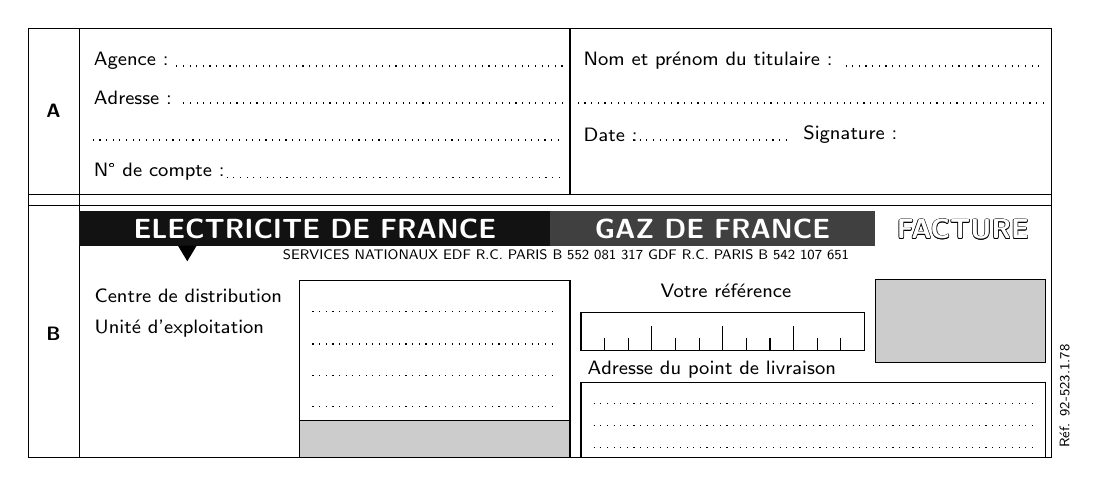
\begin{tikzpicture}[x=1cm,y=1cm,font=\sffamily\scriptsize]
\draw (0,0) rectangle (13,5.45);
\draw (.65,0)--(.65,5.45) (0,3.34)--(13,3.34) (0,3.20)--(13,3.20)
 (6.88,3.34)--(6.88,5.45);
\node at (.32,4.4) {\textbf{A}};
\node[anchor=west] at (.71,5.04) {Agence :}; \draw[dotted] (1.88,4.97)--(6.79,4.97);
\node[anchor=west] at (.71,4.57) {Adresse :}; \draw[dotted] (1.97,4.50)--(6.79,4.50);
\draw[dotted] (.82,4.03)--(6.79,4.03);
\node[anchor=west] at (.71,3.63) {N° de compte :}; \draw[dotted] (2.52,3.55)--(6.79,3.55);
\node[anchor=west] at (6.93,5.04) {Nom et prénom du titulaire :};
\draw[dotted] (10.38,4.97)--(12.89,4.97) (6.98,4.50)--(12.91,4.50);
\node[anchor=west] at (6.93,4.10) {Date :};
\draw[dotted] (7.68,4.03)--(9.69,4.03);
\node[anchor=west] at (9.72,4.10) {Signature :};
\node at (.32,1.57) {\textbf{B}};
\fill[black!93] (.65,2.69) rectangle (6.63,3.13);
\fill[black!75] (6.63,2.69) rectangle (10.75,3.13);
\node[text=white,font=\sffamily\bfseries] at (3.64,2.90) {ELECTRICITE DE FRANCE};
\node[text=white,font=\sffamily\bfseries] at (8.69,2.90) {GAZ DE FRANCE};
\foreach \dx/\dy/\ink in {-.22/0/black,-.16/.16/black,0/.22/black,.16/.16/black,.22/0/black,.16/-.16/black,0/-.22/black,-.16/-.16/black,0/0/white}{
  \node[xshift=\dx pt,yshift=\dy pt,text=\ink,font=\sffamily\bfseries] at (11.87,2.90) {FACTURE};
}
\fill (1.90,2.69)--(2.02,2.49)--(2.14,2.69)--cycle;
\node[font=\sffamily\tiny] at (6.83,2.57) {SERVICES NATIONAUX EDF R.C. PARIS B 552 081 317 GDF R.C. PARIS B 542 107 651};
\node[anchor=west] at (.72,2.05) {Centre de distribution};
\node[anchor=west] at (.72,1.63) {Unité d'exploitation};
\fill[black!20] (3.45,0) rectangle (6.88,.47);
\draw (3.45,0) rectangle (6.88,2.25) (3.45,.47)--(6.88,.47);
\foreach \y in {1.85,1.44,1.04,.65}{\draw[dotted] (3.61,\y)--(6.72,\y);}
\node at (8.86,2.11) {Votre référence};
\draw (7.02,1.36) rectangle (10.62,1.84);
\foreach \x in {7.32,7.62,8.22,8.52,9.12,9.42,10.02,10.32}{\draw (\x,1.36)--(\x,1.51);}
\foreach \x in {7.92,8.82,9.72}{\draw (\x,1.36)--(\x,1.67);}
\filldraw[fill=black!20] (10.76,1.20) rectangle (12.92,2.26);
\node[anchor=west] at (6.98,1.11) {Adresse du point de livraison};
\draw (7.02,0) rectangle (12.92,.95);
\foreach \y in {.68,.40,.12}{\draw[dotted] (7.18,\y)--(12.80,\y);}
\node[rotate=90,anchor=west,font=\sffamily\tiny] at (13.16,.00) {Réf. 92-523.1.78};
\end{tikzpicture}}}

En cas de désaccord sur le montant d'un prélèvement, je réglerai le différend directement avec EDF-GDF.

Il est entendu qu'aucun avis particulier ne me sera adressé lors de l'exécution, ou, éventuellement, de la non-exécution des prélèvements.

\begin{flushright}\small 3420\\\end{flushright}
\figure{\makebox[\linewidth][r]{
\begin{tikzpicture}[x=.19cm,y=.19cm]
\draw[line width=1.4pt] (.61,.75) .. controls (.46,.98) and (.10,.81) .. (.21,.57)
 .. controls (.30,.35) and (.48,.76) .. (.56,.43)
 .. controls (.62,.22) and (.33,.07) .. (.18,.27);
\draw (-.52,.04)--(.97,.04);
\node[anchor=north,font=\tiny] at (.36,.02) {\unsure{Sodel|Sodé}};
\end{tikzpicture}}}
% archive sheet number: 8

\scanpage{10}

1) $X$ espace topologique, $U,V$ ouverts, conditions équivalentes
\[
\begin{aligned}
\text{a)}\quad & U=\complement\overline V,\quad V=\complement\overline U\\
\text{b)}\quad & U\cap V=\varnothing,\quad\complement(U\cup V)\subset\overline U\cap\overline V
 \qquad\text{(d'où égalité.)}\\
\text{c)}\quad & U\cap V=\varnothing,\quad X=\overline{U\cup V},\quad\dot U=\dot V\\
\text{d)}\quad & \overline U\cap\overline V=\dot U=\dot V\ \unsure{\Leftarrow|?}
\end{aligned}
\]

$U$ et $V$ se déterminent mutuellem$^{\mathrm t}$. Pour $U$ fixé, il existe $V$ ayant les propriétés précédentes ssi $V=\complement\overline U$ est dense dans $\complement U$.

3) $X$ espace topologique, $K\subset X$ fermé, $U_K^{\deleted{\unsure{\prime|3}}}$ et $\deleted{\unsure{V}}U'_K$ deux ouverts relatifs de $X$ tels que
\[
\resizebox{.99\linewidth}{!}{$\displaystyle
\overline U_K^{\deleted{\unsure{\prime|-}}}=K\smallsetminus U'_K,\quad
\overline{U'_K}=K\smallsetminus U_K,\quad
C=\overline U_K\cap\overline{U'_K}=
\underset{\deleted{\overline U_K\smallsetminus U_K\unsure{=}\overline{U'_K}\smallsetminus U^{\unsure{\prime}}_K}}
 {\overset{\inserted{\overline U_K\smallsetminus U_K=\overline{U'_K}\smallsetminus U'_K}}
 {\text{frontière commune}}}$}
\]
de $U_K$ et $U'_K$ \uline{dans $K$} \inserted{(fermé dans $X$)}. Soit $B=U_K\cap\dot K$, \deleted{donc} donc $B$ ouvert ds $\dot K$ et fermé ds $U_K$ donc \unsure{rel$^{\mathrm t}$.} fermé ds $X$, Alors on a, posant \inserted{si $B\cap C=\varnothing$.}
\[
\resizebox{\linewidth}{!}{$\displaystyle\left\{\begin{aligned}
&U=U_K\smallsetminus\deleted{\unsure{D}}B_{\deleted{\unsure{K}}}=\operatorname{Int}(U_K)\\
&V=X\smallsetminus\overline U_K^{\deleted{\prime}}=
 (\underbrace{X\smallsetminus U_K}_{\inserted{X_1}})\smallsetminus C=\operatorname{Int}(X_1)\\
&U=\complement\overline V,\ V=\complement\overline U,\qquad
 \dot U=\dot V=\overline U\cap\overline V=\complement(U\cup V)=B\cup C\\
&\deleted{U\cap K=U\subset K,\ V\cap K=V_K}\quad
 \underbrace{V\subset X_1}_{\inserted{\text{diff. }C}}
 \underbrace{{}\subset\overline V}_{\inserted{\text{diff }B}}
\end{aligned}\right.$}
\]

\uline{Cor} \deleted{Si $B\cap C=\varnothing$ i.e. $U_K\smallsetminus U$, Supposons} \inserted{Pour que} \deleted{$B$} $X_1=\complement U_K$ soit loc fermé, il f. et s. que $B=U_K\cap\dot K$ soit \deleted{fermé dans $X$, \unsure{alors}} \deleted{\unsure{dans} $B\cup$} \deleted{$B$ est ouvert et} fermé dans $X$, ou encore que ce soit un sommand \unsure{topolog} \deleted{dans $\dot K$, et posant $K=B'\amalg B$} \deleted{\unsure{de|sur} $\dot K$. Posant alors $\dot K=B'\amalg \unsure{B|B'}$} ou encore qu'il soit fermé ds $B\cup C$, ou encore que $\overline B\cap C=\varnothing$. [Il suffit pour ceci que $\dot K\cap C=\varnothing$ i.e. que $U_K\unsure{\cup|\amalg}V_K\supset K^{\bullet}$]. \deleted{i.e. $U_K$ et $V_K$ sont}
% archive sheet number: 9

\scanpage{11}
% archive sheet number: 10
% The calculation on the left half turns through 180 degrees.
\[
\begin{aligned}
t^2(\lambda_0)&=\lambda_0\\
t^2(\lambda_1)&=t(\unsure{q|g}_{\unsure{\nu|v}})\underbrace{t(\lambda_{\unsure{\nu|v}})}_{\lambda_1}t(\unsure{q|g}_{\unsure{\nu|v}})^{-1}
\end{aligned}
\]

\[
\lambda_0\quad\lambda_1\quad\lambda_2
\qquad\qquad \text{\uline{$t^2=\mathrm{int}$}}(\lambda_0)
\]
\[
\begin{aligned}
t(\lambda_0)&=\lambda_0\\
t(\lambda_1)&=\lambda_1\lambda_2\lambda_1^{-1}=\lambda_0^{-1}\lambda_2\lambda_0\\
t(\lambda_2)&=\lambda_1
\end{aligned}
\]

\[
\begin{aligned}
t^2(\lambda_0)&=\lambda_0\\
t^2(\lambda_1)&=(\lambda_1\lambda_2\deleted{\lambda_1^{-1}})\deleted{\lambda_1}
   (\lambda_1\lambda_2^{-1}\lambda_1^{-1})\\
 &=\lambda_1\underbrace{\lambda_2\lambda_1\lambda_2^{-1}}\lambda_1^{-1}\\
 &=\mathrm{int}(\lambda_1,\lambda_2)\lambda_1
   =\mathrm{int}(\lambda_0^{-1})\lambda_1\\
t^2(\lambda_2)&=t(\lambda_1)=\lambda_1\lambda_2\lambda_1^{-1}
   =\deleted{\mathrm{int}(\lambda_1})\\
 &=(\lambda_1\lambda_2)\lambda_2(\lambda_2^{-1}\lambda_1^{-1})\\
 &=\mathrm{int}(\lambda_{\unsure{1|0}}\lambda_2)\lambda_2\,\mathrm{int}(\lambda_1
\end{aligned}
\]
% Detached short pen stroke beside the last line on the rotated half.
\margin{$\unsure{\prime|\cdot}$}

% Upright half of the sheet.
\diagram{\begin{tikzcd}[ampersand replacement=\&,column sep=large]
\deleted{\unsure{A|H}}\,G/H
 \& \widetilde E=\unsure{G|\mathbb G}\unsure{\wedge|\times}_{H}\unsure{E|\mathbb E} \arrow[l]\arrow[d]
 \& G\times_{H}E\arrow[l]\arrow[d]\\
 e\arrow[u,no head]\arrow[r,no head]
 \& E\arrow[ul] \& E'\arrow[l]
\end{tikzcd}}

\diagram{\begin{tikzcd}[ampersand replacement=\&,column sep=small,row sep=large]
 B_H \arrow[d,"f"',no head] \& E_H
 \& \vphantom{E}\arrow[d,no head,start anchor=north,end anchor=south] \& f_! f^{*}(E)\arrow[r] \& E\arrow[l,bend right=20,dashed]\\
 B_G- \& E' \& \vphantom{E}
 \& f^{*}f_!(f^{*}E)\arrow[r]
 \& f^{*}E\arrow[l,bend left=20]
\end{tikzcd}}

\[
\widetilde E\simeq
\]

\scanpage{12}
% archive sheet number: 11
3) Supposons $\dot K\cap C=\emptyset$, et posons
\[
\begin{aligned}
 \unsure{\cdot|{}}B'&=U'_K\cap\dot K\\
 U'&=U'_K\setminus B'=\mathrm{Int}(U'_K)\\
 V'&=X\setminus\overline{U'_K}=(\underbrace{X\setminus U'_K}_{X'_1})\setminus C\\
   &=\mathrm{Int}(X'_1)
\end{aligned}
\]
\[
\deleted{U'=U'_K}
\]
enfin $W=V\cap V'=\complement K$.

\diagram{\begin{tikzcd}[ampersand replacement=\&,row sep=large,column sep=small]
 U^{\deleted{\unsure{'|1}}}\arrow[dr,no head,"B"'] \& \& U'\arrow[ll,"C"']\arrow[dl,no head,"B'"']\\
 \& W^{\deleted{U}} \&
\end{tikzcd}}

\figure{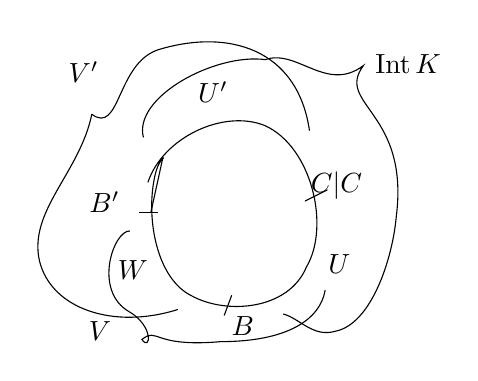
\begin{tikzpicture}[x=0.95cm,y=0.95cm]
\draw (0.88,3.06) .. controls (1.26,2.78) and (1.21,3.73) .. (1.76,3.92)
 .. controls (2.7,4.21) and (3.63,3.94) .. (3.79,2.84);
\draw (0.88,3.06) .. controls (0.72,2.28) and (0.03,1.77) .. (0.18,1.1)
 .. controls (0.34,0.45) and (1.18,0.18) .. (2.03,0.45);
\draw (1.57,2.75) .. controls (1.43,3.29) and (2.53,3.88) .. (3.20,3.79)
 .. controls (3.62,3.94) and (4.02,3.34) .. (4.51,3.71)
 .. controls (4.13,3.19) and (5.13,3.10) .. (4.95,1.69)
 .. controls (4.9,1.13) and (4.62,0.26) .. (4.14,0.16)
 .. controls (3.84,0.07) and (3.66,0.33) .. (3.44,0.39);
\draw (1.39,1.5) .. controls (1.17,1.51) and (0.89,0.70) .. (1.38,0.42)
 .. controls (1.72,0.22) and (1.66,-0.12) .. (1.55,0.05)
 .. controls (1.77,0.22) and (1.68,-0.06) .. (2.60,0.02)
 .. controls (3.47,0.02) and (3.93,0.30) .. (4.00,0.71);
\draw (1.63,2.15) .. controls (1.83,2.75) and (2.64,3.13) .. (3.19,2.91)
 .. controls (3.82,2.63) and (4.07,1.56) .. (3.75,1.02)
 .. controls (3.51,0.44) and (2.68,0.38) .. (2.22,0.63)
 .. controls (1.76,0.85) and (1.61,1.62) .. (1.71,2.17)
 .. controls (1.74,2.34) and (1.78,2.42) .. (1.84,2.48);
\draw (1.83,2.48)--(1.67,1.75);
\draw (1.51,1.75)--(1.76,1.75);
\draw (3.73,1.90)--(4.03,2.05);
\draw (2.75,0.64)--(2.65,0.37);
\node at (0.77,3.62) {$V'$}; \node at (2.50,3.36) {$U'$};
\node[right] at (4.54,3.73) {$\mathrm{Int}\,K$};
\node at (1.05,1.89) {$B'$}; \node at (4.15,2.11) {$\unsure{C|\mathbb C}$};
\node at (1.43,0.98) {$W$}; \node at (4.19,1.06) {$U$};
\node at (0.99,0.16) {$V$}; \node at (2.90,0.23) {$B$};
\end{tikzpicture}}

Alors on a :
\[
\begin{array}{ll|l}
 U,U',W&\text{ouverts disjoints}& U,U',W,B,B',C\\
 B,B',C&\text{fermés disjoints}&\text{pseudopartition de }X
\end{array}
\]
\[
\left\{\begin{aligned}
 &\overline U\cap\overline{U'}=C,\quad
 \overline U^{\deleted{\unsure{'|*}}}\cap\overline W=B,\quad
 \overline W\cap\overline{U'}=B'\\
 &\unsure{\dot U'|\overline{U'}}\deleted{\unsure{\setminus|{}}}=\overline{U'}\setminus U'=B'\cup C,\quad
 \dot U=B\cup C,\quad \dot W=B\cup B'\\
 &K=\overline{U\cup U'}=\complement W=(U\cup U')\cup B\cup B'\cup C,\quad
 \mathrm{Int}\,K=(U\cup U'\cup C
\end{aligned}\right.
\]
\deleted{\illegible{1}}

4) \deleted{Donnons} Soient $U,U',W$ 3 ouverts d'un espace $X$.

Conditions équivalentes

a) $U,U',W$ mutuellement disjoints, réunion dense,
\[
 \overline U\cap\overline{U'}\cap\overline W=\emptyset,\quad
 \deleted{\unsure{\overline U|U}\unsure{\cap}}\dot U\subset\overline{U'\cup W},\quad
 \dot U'\subset\overline{U\deleted{\unsure{\cap|'}}\cup W},\quad
 \dot W\subset\overline{U\cup U'}
\]

b) Posant $C=\overline U\cap\overline{U'}$, $B=\overline U\cap\overline W$, $B'=\overline W\cap\overline{U'}$, les 6 ens $U,U',W,B,B',C$ forment une pseudopartition de $X$.

On a alors les relations ci-dessus --

Il revient au $=$ de se donner (pour $X$ fixé) $U,U',W$ satisfaisant les conditions \inserted{équ.} a) b), ou $K,$ \inserted{fermé de $X$} et $\underbrace{U_K,U'_K}_{\text{ouverts de }K}$ satisfaisant
\[
\left\{\begin{aligned}
 \overline{U_K}&=K\setminus U'_K,\quad \overline{W_K}=K\setminus U_K\\
 C\cap\dot K&=\emptyset\quad \text{où}\quad C=\overline{U_K}\cap\overline{U'_K}=K\setminus(U_K\cup U'_K)
\end{aligned}\right.
\]

\scanpage{13}
% archive sheet number: 12
% A fine diagonal stroke crosses the writing from the upper D(d) down
% to the last group. The last group is also crossed by short diagonals.
\diagram{\deleted{\mbox{\begin{tikzcd}[ampersand replacement=\&,column sep=small,row sep=large,font=\footnotesize]
d \& D(d)=\pi_0\Sigma_d(\unsure{\mathfrak X|\mathscr X|\mathcal X|X})
 \arrow[r,"{\overset{\alpha_d}{\sim}}"]\arrow[d,"{R_{d',d}}"]
 \& E(d)\overset{\text{dfn}}{=}\{e\in E\mid\varphi(M(e))=d\}
 \arrow[d,"{r_{d',d}}"]\\
 \shortstack{$\cup$\\$d'$} \& D(d')\arrow[r,"{\overset{\alpha_{d'}}{\sim}}"]
 \& E(d')
\end{tikzcd}}}}

\diagram{\deleted{\mbox{\begin{tikzcd}[ampersand replacement=\&,column sep=small,row sep=small,font=\footnotesize]
D(\{i\})=\pi_0[\deleted{\Delta}\Sigma(X_i,\partial X_i)
 \arrow[r,"{\overset{\alpha_i}{\sim}}"]
 \& E(\{i\})=\varphi^{-1}(\{i\})\\
 \begin{array}{cc}\Vert&\backslash\\[-2pt]
 \displaystyle\bigcup_{\mu\varphi(M(e))\le i}|E_e|,
 &\displaystyle\bigcup_{\mu\varphi\unsure{\lvert|(}M(e)<i}(E_e\rvert
 \end{array} \&
\end{tikzcd}}}}

\[
\deleted{\partial X_i=\bigcup_{\mu(\varphi(M(e)))<i}|E_e|}
\]
\[
\deleted{\partial X_i\overset{\text{dfn}}{=}\bigcup_{j<i}X_j
 =\bigcup_{j<i}\ \bigcup_{\substack{e\in E\\\varphi M e)\le j}}|E_e|
 =\bigcup_{\substack{e\in E\\\exists\,j\ \text{tel que}\\\varphi\mathord{.}(M\mathord{.}(e))\le j<i}}|E_e|}
\]
\figure{
\begin{tikzpicture}[x=0.7cm,y=0.7cm]
\draw (0,0) .. controls (2.8,0.09) and (3.0,0.06) .. (3.95,0.30)
 .. controls (4.32,0.38) and (3.91,-0.17) .. (4.33,-0.16)
 .. controls (6.6,-0.05) and (9.9,-0.10) .. (12.1,0.08);
\end{tikzpicture}}

\[
\deleted{|\unsure{\mathcal K|K|k}|=(K_0,K)\supset(L_0,L)=|L|}
\qquad\mathrel{.\mkern2mu:}
\]
\diagram{\deleted{\mbox{\begin{tikzcd}[ampersand replacement=\&,row sep=tiny,column sep=0pt]
 \& \deleted{\unsure{\alpha|x}}\arrow[d,bend left=14] \&\\
 \&\deleted{\unsure{X|K}}\&\\
 \Sigma \& ( \& |K|,|L|)=|\Delta|
\end{tikzcd}}}}
\[
\deleted{\widetilde{\deleted{K}\Delta}\overset{\text{dfn}}{=}
 \Sigma(K,L)=(\widetilde{\deleted{K}\Delta}_0,\widetilde{\deleted{K}\Delta})}
\]
\[
\deleted{\left\{\begin{aligned}
 \widetilde{\deleted{K}\Delta}_0&=\varinjlim_{\sigma\in K\setminus L}
 \underset{\cdot}{\sigma}\;(\subset{\deleted{\Delta}K}_0)\xrightarrow{\pi}{\deleted{\Delta}K}_0\\
 \widetilde{\deleted{K}\Delta}&=\mathrm{Im}\bigl((K\setminus L)\longrightarrow
 \mathcal P(\Delta_0)\bigr)
\end{aligned}\right.}
\]

\diagram{\deleted{\mbox{\begin{tikzcd}[ampersand replacement=\&,row sep=small,column sep=small]
 \deleted{\unsure{\Sigma|E}}|\widetilde{\deleted{K}\Delta}|\arrow[r,"?"]
 \& \Sigma(|K|,|L|)\\
 \Vert \& \sigma'=\mathrm{Im}(\sigma) \& \underline{\sigma}\in K\setminus L\\
 \displaystyle\varinjlim_{\sigma'\in\Delta}|\sigma'| \&
 |\sigma|\arrow[r]\arrow[rr,bend right=12] \& |\sigma'|\arrow[r] \& \Sigma
\end{tikzcd}}}}

\scanpage{14}
% archive sheet number: 13
\[
\begin{aligned}
 \Gamma_1&:\Gamma'_2\cup\Gamma'_3\\
 \Gamma_2&=\Gamma'_3\cup\Gamma'_1\\
 \Gamma_3&:\Gamma'_1\cup\Gamma'_2
\end{aligned}
\]

\diagram{\begin{tikzcd}[ampersand replacement=\&,column sep=small,row sep=small,font=\small]
 \& {\begin{gathered}\mathrm{a)}\quad\unsure{v|\nu}_1,v_2,v_3\\
 \text{\deleted{appartiennent}\inserted{contenus} dans}\\
 \text{régions distinctes}\\[-2pt]\text{de }E-\Gamma\end{gathered}}
 \arrow[d,Rightarrow] \\
 {\begin{gathered}\mathrm{a}')\ E-\Gamma\text{ a}\\
 \text{trois régions}\\\text{distinctes}\end{gathered}}\arrow[ur,Leftrightarrow]
 \& {\begin{gathered}\mathrm{b)}\quad\Gamma_1,\Gamma_2,\Gamma_3\text{ sont des courbes de}\\
 \text{Jordan}\end{gathered}}\arrow[d,Rightarrow]\\
 \&{\begin{gathered}\mathrm{c)}\quad\Gamma_1,\Gamma_2\text{ sont des courbes}\\
 \text{de Jordan}\end{gathered}}
\end{tikzcd}}

\figure{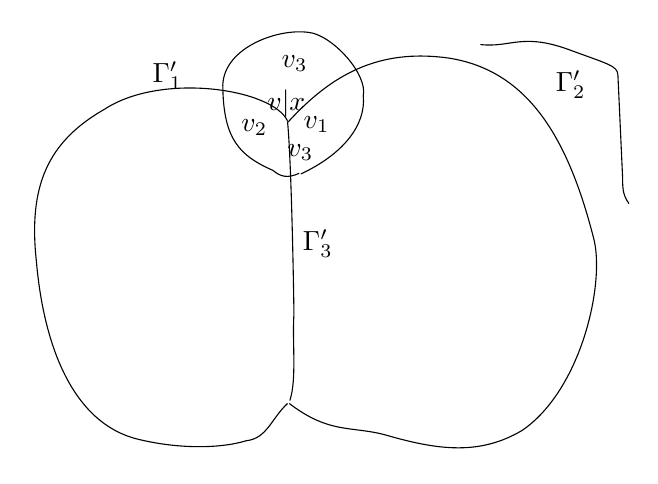
\begin{tikzpicture}[x=0.74cm,y=0.74cm]
\draw (4.34,5.59) .. controls (4.08,6.14) and (2.18,6.43) .. (1.20,5.79)
 .. controls (0.22,5.23) and (-0.11,4.47) .. (0.03,3.18)
 .. controls (0.16,1.68) and (0.68,0.40) .. (1.76,0.13)
 .. controls (2.44,-0.04) and (3.17,-0.04) .. (3.63,0.10)
 .. controls (3.99,0.14) and (4.06,0.48) .. (4.34,0.74);
\draw (4.35,5.57) .. controls (5.10,6.39) and (5.90,6.83) .. (7.09,6.67)
 .. controls (8.49,6.46) and (9.16,5.26) .. (9.59,3.59)
 .. controls (9.80,2.83) and (9.39,0.98) .. (8.37,0.28)
 .. controls (7.65,-0.15) and (6.94,-0.06) .. (6.09,0.18)
 .. controls (5.47,0.37) and (5.09,0.19) .. (4.37,0.74);
\draw (4.34,5.58) .. controls (4.40,4.97) and (4.44,3.09) .. (4.45,2.28)
 .. controls (4.42,1.76) and (4.50,1.16) .. (4.38,0.79);
\draw (4.57,4.68) .. controls (5.28,5.01) and (5.69,5.51) .. (5.64,6.02)
 .. controls (5.72,6.40) and (5.09,7.08) .. (4.69,7.11)
 .. controls (4.14,7.18) and (3.19,6.82) .. (3.23,6.14)
 .. controls (3.25,5.27) and (3.52,4.99) .. (4.09,4.74)
 .. controls (4.22,4.63) and (4.34,4.60) .. (4.54,4.69);
\draw (7.65,6.90) .. controls (8.18,6.84) and (8.37,7.12) .. (9.23,6.79)
 .. controls (9.86,6.56) and (10.00,6.53) .. (10.01,6.38)
 --(10.09,4.63) .. controls (10.09,4.41) and (10.10,4.31) .. (10.20,4.17);
\node at (2.28,6.36) {$\Gamma'_1$};
\node at (9.20,6.21) {$\Gamma'_2$}; \node at (4.86,3.48) {$\Gamma'_3$};
\node at (4.46,6.58) {$v_3$}; \node at (3.77,5.47) {$v_2$};
\node at (4.84,5.52) {$v_1$}; \node at (4.32,5.88) {$\deleted{\unsure{v|x}}$};
\node at (4.56,5.05) {$\deleted{v_3}$};
\end{tikzpicture}}

\[
\begin{aligned}
 &\mathrm{a)}\longleftrightarrow\mathrm{a}')\\
 &\mathrm{b)}\Longrightarrow\mathrm{c)}\deleted{\unsure{\Rightarrow|\Leftrightarrow}}\ \text{triv.}\\
 &\mathrm{c)}\Longrightarrow\mathrm{a)}
\end{aligned}
\]

\deleted{\unsure{En suivant|En entourant} $\Gamma'_3$ \unsure{on dit}}
Car 2 pts de part et d'autre de $\Gamma'_3$ \deleted{\unsure{sont}} \unsure{doivent}
\unsure{être} ds des régions distinctes de $E-\Gamma_1$
(\inserted{\unsure{ou}} $E-\Gamma_2$), \unsure{sont} \inserted{à fortiori} \unsure{alors} régions distinctes de
\deleted{\inserted{$\unsure{E'|E}$}$E-\unsure{\Gamma_1\cup\Gamma_2|\Gamma_2}$}
\inserted{$=E-\Gamma$}, donc $v_1$ et $v_2$ sont des régions distinctes.
De $=$, deux pts de part et d'autre de $\Gamma'_1$ \inserted{($\Gamma'_2$)}
sont des régions distinctes de $E-\Gamma_2$ ($E-\Gamma_1$) donc sont des régions distinctes
dans $E-\Gamma$, OK.

$\mathrm{a)}\longrightarrow\mathrm{b)}$\qquad Prouvons que $\Gamma_3$ (p.ex.) est courbe de Jordan.

\scanpage{15}
% archive sheet number: 14
% letterhead
\noindent\begin{tabular}[t]{@{}c@{}}
U N I V E R S I T E\\
DES SCIENCES ET TECHNIQUES\\
DU LANGUEDOC\\
\textasciicircum\textasciicircum\textasciicircum\textasciicircum\textasciicircum\textasciicircum\textasciicircum\textasciicircum\textasciicircum\textasciicircum\textasciicircum\textasciicircum\\[3pt]
Service de la Scolarité\\
JP/GJ\\[3pt]
\uline{Diffusion} : Liste A\\
N\textdegree{}2417
\end{tabular}\hfill\begin{tabular}[t]{@{}l@{}}
MONTPELLIER, le 19 AVRIL 1977\\
\end{tabular}

% printed form
\begin{center}
\uline{AVIS DE SOUTENANCE D'UNE THESE DE DOCTORAT DE}\\[3pt]
\uline{SPECIALITE : CHIMIE Mention CHIMIE-PHYSIQUE}
\end{center}

\uline{Nom et prénom du candidat} : BERLANDIER Gaston

\uline{Titre de la thèse} : Etude comparée des spectres de vibration de
\[
\mathrm{CH}_{3}\text{-}\mathrm{C}\hphantom{\mathrm{CC}}\mathrm{Cl}_{2}\text{-}\mathrm{CH}_{3},\quad
\mathrm{CD}_{3}\text{-}\mathrm{C}\hphantom{\mathrm{C}}\mathrm{Cl}_{2}\text{-}\mathrm{CD}_{3}
\quad\text{et}\quad\mathrm{CD}_{3}\text{-}\mathrm{CCl}_{2}\text{-}\mathrm{CH}_{3}
\]

\uline{Date, heure et lieu de soutenance prévus} : 23 AVRIL 1977 à 10 heures, Salle de Cours n\textdegree{} 10 - U.S.T.L.

\uline{Nom du Directeur de thèse} : Messieurs BRIBES et GAUFRES

\uline{Désignation du laboratoire où la thèse est préparée} : Laboratoire de Spectroscopie Moléculaire de l'Université des Sciences et Techniques du Languedoc.

\uline{Analyse de l'ouvrage} : Après avoir décrit la préparation des composés deutérés, ainsi que le contrôle de leur pureté isotopique, l'auteur présente et analyse les spectres de vibration des trois espèces, à savoir les spectres d'absorption et de diffusion des phases liquide et gazeuse. L'identification des fréquences fondamentales repose sur les formes des enveloppes des bandes en infrarouge comme en Raman, ainsi que sur le facteur de dépolarisation en diffusion. La recherche de la meilleure attribution compte tenu de la règle du produit et des informations expérimentales est faite systématiquement par ordinateur. 73 fréquences fondamentales sur 81 sont données avec une bonne certitude.

\uline{Durée approximative des recherches ayant abouti à la thèse} : Deux ans

\uline{Composition du jury proposé} :
\begin{center}
\begin{tabular}{@{}lll@{}}
MM. : & R. & GAUFRES\\
 & J. & PETRISSANS\\
 & J.L. & BRIBES\\
 & P. & SAUMAGNE\\
 & V. & TABACIK
\end{tabular}
\end{center}

\begin{flushright}
Le Secrétaire Général,\\
\handwritten{\unsure{E S|E Siau}}\\
\uline{E. SIAU}\\
\end{flushright}

\scanpage{17}
% archive sheet number: 16
\figure{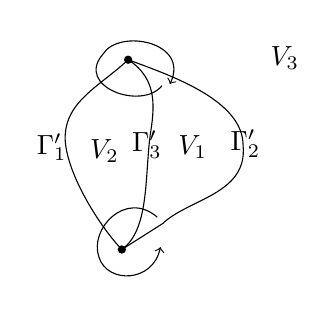
\begin{tikzpicture}[x=1cm,y=1cm]
\draw (1.08,2.56) .. controls (0.72,2.22) and (0.27,2.03) .. (0.28,1.55)
 .. controls (0.30,1.10) and (0.73,0.43) .. (1.00,0.15);
\draw (1.08,2.56) .. controls (1.47,2.31) and (1.41,1.93) .. (1.36,1.60)
 .. controls (1.29,1.07) and (1.35,0.40) .. (1.00,0.15);
\draw (1.08,2.56) .. controls (1.65,2.35) and (2.54,2.04) .. (2.54,1.47)
 .. controls (2.60,0.85) and (1.84,0.79) .. (1.52,0.48) -- (1.00,0.15);
\draw[->] (1.51,2.23) .. controls (1.25,1.91) and (0.40,2.22) .. (0.76,2.63)
 .. controls (0.96,2.96) and (1.87,2.79) .. (1.61,2.25);
\draw[->] (1.45,0.56) .. controls (1.05,0.91) and (0.58,0.41) .. (0.71,0.05)
 .. controls (0.82,-0.29) and (1.40,-0.27) .. (1.49,0.18);
\fill (1.08,2.56) circle (1.5pt); \fill (1.00,0.15) circle (1.5pt);
\node at (0.11,1.45) {$\Gamma'_1$}; \node at (0.78,1.40) {$V_2$};
\node at (1.32,1.48) {$\Gamma'_3$}; \node at (1.90,1.45) {$V_1$};
\node at (2.57,1.49) {$\Gamma'_2$}; \node at (3.07,2.58) {$V_3$};
\end{tikzpicture}}

$\Gamma'_i\qquad \alpha\in I$ ens \unsure{à|:} trois él.
chemin simple joignant les deux point de $\delta=\{x,y\}$

$\Gamma_i=\displaystyle\bigcup_{\underline{j}\in A-\{i\}}\Gamma'_j$
détermine un ens $B_i$ de card. 2 (\unsure{l'une|l'un} des 2 régions du \deleted{\unsure{pl.}}\inserted{$X$})

\[
 B=\coprod_{i\in I} B_i\qquad
 \text{\deleted{\unsure{:|.} \unsure{quotient|points|graphe} de 3 côtés}}
\]

Si $i\in I$ est donné, on lui associe $U_i$ la région de $\Gamma_i$ qui contient $\Gamma'_i-\delta$ \inserted{$=\Gamma_i^{\prime\circ}$}, d'où section de la \unsure{sur. quelle|surj. quelle|sur quelle}
\[
 B\simeq I\times\{0,1\},\qquad V_i
\]

\[
\begin{aligned}
 U_i&=\overset{\circ}{\Gamma}'_i\cup\bigcup_{j\in I\setminus\{i\}}U_j\\
 V_i&=\bigcap_{j\in I\setminus\{\unsure{i|1}\}}V_j
\end{aligned}
\qquad\Bigg/\qquad
\left\{\begin{gathered}
 V_1,V_2,V_3\\ \Gamma_1^\circ,\Gamma_2^\circ,\Gamma_3^\circ\\ \delta
\end{gathered}\right.
\quad
\left\{\begin{aligned}
 U_1&=V_2\cup V_3\cup\Gamma_1^\circ\\
 U_2&=V_3\cup V_1\cup\Gamma_2^\circ\\
 U_3&=V_1\cup V_2\cup\Gamma_3^\circ
\end{aligned}\right.
\]
\[
 U_i,U_j,\ U_k\qquad\Bigg/\qquad
\begin{aligned}
 V_3&=U_1\cap U_2\\
 V_2&=U_3\cap U_1\\
 V_1&=U_1\cap U_2
\end{aligned}
\quad
\left\{\begin{aligned}
 \Gamma_1&=\Gamma_2^\circ\cup\Gamma_3^\circ\cup\delta\\
 \Gamma_2&=\Gamma_3^\circ\cup\Gamma_{\unsure{1|2}}^\circ\cup\delta\\
 \Gamma_3&=\Gamma_1^\circ\cup\Gamma_2^\circ\cup\delta
\end{aligned}\right.
\]

$C$ courbe simple fermée dans surface connexe \deleted{$X$}$E$. Conditions équ.

a) card $\pi_0(\deleted{X}E-C)=2$ \quad (\uline{NB} on a tjrs card $\pi_{\unsure{0|{}}}(E-C)\le 2$)

b) $\exists$ ouvert $U\subset C$ tel que $\dot U(\overset{\text{dfn}}{=}\overline U-U)=C$ et que \deleted{\unsure{vide|de}}
$\overline U\ne E$ i.e. $V=\overline U-U\ne\emptyset$ i.e. $U\ne E\setminus C$.
% slanted
\margin{($U$ est alors une comp. connexe de $X-C$)}

c) (étant donné un disque $D_x$ assez petit \unsure{centré|\deleted{centré}} en $x\in C$\}, et un point $x'$ et un point $x''$ $\in D_x-D_x\cap C$ de part et d'autre de $D_x\cap C$ ....)
$x$ et $y$ n'appart\unsure{iennent|\deleted{iennent|ent}} \unsure{pas|ps.} à la $=$ composante connexe de $X-C$, i.e. $\nexists$ arc \unsure{dans|ds} $X-C$ joignant $x$ : $y$.
(Car $\{x,y\}\longrightarrow\pi_0(X-C)$ est surjectif ...)

\scanpage{19}
% archive sheet number: 18
\uline{Proposition}\qquad Soient $\Gamma,\Gamma'$ deux J.polygônes \unsure{sur|du} plan $E$, tels que $\Gamma\cap\Gamma'=I$ soit un arc polygonal non réduit \unsure{à|:} un point. Alors on est dans l'un des deux cas suivants (s'excluant mutuellement)

\[
\begin{aligned}
 &\mathrm{a)}\quad \Gamma-I\subset\mathrm{Ext}(\Gamma'),\quad
 \Gamma'-I\subset\mathrm{Ext}(\Gamma)\\
 &(\Longleftrightarrow\quad \mathrm{Int}\,\Gamma'\subset\mathrm{Ext}\,\Gamma,\quad
 \mathrm{Int}\,\Gamma\subset\mathrm{Ext}\,\Gamma')
\end{aligned}
\]
\[
\begin{aligned}
 &\mathrm{b)}\quad\Gamma-I\subset\mathrm{Ext}\,\Gamma',\quad
 \Gamma'-I\subset\mathrm{Int}\,\Gamma\quad \text{(ou inversement)}\\
 &(\Longleftrightarrow\quad \mathrm{Int}\,\Gamma'\subset\mathrm{Int}\,\Gamma,\quad
 \mathrm{Ext}(\Gamma)\subset\mathrm{Ext}\,\Gamma'\quad \text{(ou inv.)})
\end{aligned}
\]

\deleted{\unsure{a)|$\alpha$)} Dans le cas a),}
Soit $\Gamma''=(\Gamma\cup\Gamma')-(I\unsure{\setminus|-}\partial I)
=\overline{\Gamma-I}\cup\overline{\Gamma'-I}$, qui est un polygône.
C'est un J-polygône, et \unsure{on a} :

\[
\begin{aligned}
 \text{\uline{Cas a)}}\quad \mathrm{Int}\,\Gamma''&=\mathrm{Int}\,\Gamma\cup\mathrm{Int}\,\Gamma'\cup(I-\partial I)\\
 \mathrm{Ext}\,\Gamma''&=\mathrm{Ext}\,\Gamma\cap\mathrm{Ext}\,\Gamma'
\end{aligned}
\]
% The circled item in the second line is carried up to the gap after en.
\noindent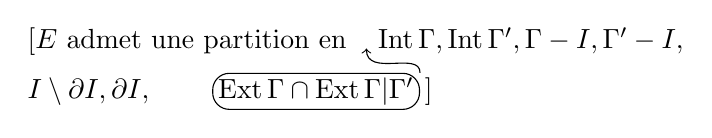
\begin{tikzpicture}[baseline=(lead.base)]
\node[anchor=base west,inner sep=0pt] (lead) at (0,0) {[$E$ admet une partition en};
\node[anchor=base west,inner xsep=2pt,inner ysep=1.5pt,draw,rounded corners=6pt]
 (moved) at (2.35cm,-1.8em)
 {\inserted{$\mathrm{Ext}\,\Gamma\cap\mathrm{Ext}\,\unsure{\Gamma|\Gamma'}$}};
\node[anchor=base west,inner sep=0pt] at ([xshift=1.1em]lead.base east)
 {$\mathrm{Int}\,\Gamma,\mathrm{Int}\,\Gamma',\Gamma-I,\Gamma'-I,$};
\node[anchor=base west,inner sep=0pt] at (0,-1.8em) {$I\setminus\partial I,\partial I,$};
\node[anchor=base west,inner sep=0pt] at ([xshift=.15em]moved.base east) {]};
\draw[->] (moved.north east) .. controls +(0,.8em) and +(0,-1.05em)
 .. ([xshift=.7em]lead.base east);
\end{tikzpicture}

\[
\begin{aligned}
 \text{\uline{Cas b)}}\quad \mathrm{Int}\,\Gamma''&=
 \mbox{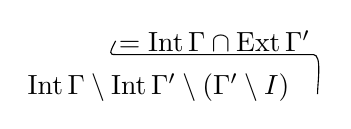
\begin{tikzpicture}[baseline=(mainterm.base)]
 \node[anchor=base west,inner sep=0pt] (mainterm) at (0,0)
 {$\mathrm{Int}\,\Gamma\setminus\mathrm{Int}\,\Gamma'\setminus(\Gamma'\setminus I)$};
 \node[anchor=base east,inner sep=1pt] (addition)
 at ([xshift=.85em,yshift=1.55em]mainterm.base east)
 {$\inserted{=\mathrm{Int}\,\Gamma\cap\mathrm{Ext}\,\Gamma'}$};
 \draw (addition.west) .. controls +(-.23em,-.45em) and +(-.24em,0) .. (addition.south west)
 -- (addition.south east) .. controls +(.32em,0) and +(0,.42em)
 .. ([xshift=1em]mainterm.base east);
 \end{tikzpicture}}\\
 \mathrm{Ext}\,\Gamma''&=\mathrm{Ext}\,\Gamma\cup\mathrm{Int}\,\Gamma'\cup(I\setminus\partial I)
\end{aligned}
\]
[$E$ admet une partition en \inserted{$\mathrm{Ext}\,\Gamma$}
$\mathrm{Int}\,\Gamma\cap\mathrm{Ext}\,\Gamma',\mathrm{Int}\,\Gamma',$
\deleted{$\mathrm{Ext}\,\Gamma$}
$\Gamma-I,\Gamma'-I,I-\partial I,\partial I$]

\scanpage{21}\mspage{I}
Le théorème de Jordan et l'existence de trois bons sommets pour un polygone \tikz[baseline=(a.base)]{\node[inner sep=1pt] (a) {de $\mathbb{R}^{2}$.};\draw[thin,gray,rotate around={8:(a.center)}] (a.center) ellipse (0.65cm and 0.30cm);}\inserted{plan}

\hspace*{\fill}Carlos C.~\unsure{Contou|Coutou}-Carrère\hspace*{\fill}

\margin{$\bullet$}On se propose de prouver les deux théorèmes suivantes :

\uline{Théorème} 1 (Jordan). Tout polygone $\Gamma$ est un $J$-polygone (cf. def 1)\margin{\tikz{\draw[gray,thin] (.1,.6) .. controls (-.2,.9) and (-.15,.1) .. (.25,-.3);\draw[gray,thin] (.25,-.35) .. controls (.35,-.6) and (.5,-.8) .. (.7,-.9);}}

\uline{Théorème} 2 (Dehn (?) non-publié). Si $\Gamma$ est un polygone, il existe au moins trois bons sommets (cf. def.\hspace{1em}) dont deux au moins sont tels que les triangles correspondants soient \unsure{interieurs|inteieurs|intérieurs}, i.e. contenus dans $\mathrm{int}_{\Gamma}\cup\Gamma$ (cf. def 2).

1- \uline{Preliminaires}

\margin{$\bullet\ \bullet$}On entend par polygone la réalisation \uline{géom}étrique dans \uline{$\mathbb{R}^{2}$} \margin{\tikz{\draw[gray,thin] (0,0) .. controls (.6,.35) and (1.15,.38) .. (1.5,.2);\draw[gray,thin] (.1,-.05) .. controls (.8,-.15) and (1.55,-.3) .. (2,-.7);}}d'un \margin{$\bullet$}polygo\uline{ne abs}trait, connexe\inserted{et non vide}. Si $\Gamma$ est un polygone on dénote par \margin{$\bullet$}$S(\Gamma)$ (resp. $A(\Gamma)$) l'ensemble des sommets (resp. arêtes) gé\uline{ometriq}\unsure{ues} de $\Gamma$.

\margin{$\cdot\quad\cdot$}Le terme ar\uline{c de} polygone désigne la réalisation \uline{géo}metrique dans $\mathbb{R}^{2}$ d'un 1-complexe connexe$\langle$ \margin{or. ?}tel que chaque sommet soit incident à 1 ou à 2 arêtes, et tel qu'il existe exactement 2 sommets qui sont incidents à une seule arête (pas néc. la même).

On appelle extrémités \unsure{d'eun|d'un|deun} arc de polygone les points de $\mathbb{R}^{2}$ qui correspondent à ces deux sommets. Si $\Gamma_{xy}$ est un arc de polygone d'\unsure{extremités|extrémités} $x,y$ on dénote par $S(\Gamma_{xy})$ (resp. $A(\Gamma_{xy})$) l'ensemble de ses sommets (resp. arêtes) géometriques.

\margin{$\bullet$}Par $\Gamma$ (resp. $\Gamma_{xy}$) on dénote a\uline{us}si l'ensemble \inserted{de $\mathbb{R}^{2}$} sous jacent à $\Gamma$ (resp. $\Gamma_{xy}$) si $\Gamma$ \deleted{est} (resp. $\Gamma_{xy}$) est un polygone (resp. arc de polygone).

\tikz[baseline=(r.base)]{\node[inner sep=1pt] (r) {\uline{Remarque 1}};\draw[dashed,gray,line width=.2pt] ([xshift=-1pt,yshift=1pt]r.north east)..controls ([yshift=5pt]r.north) and ([xshift=-3pt,yshift=4pt]r.north west)..([xshift=-3pt]r.west)..controls ([xshift=-3pt,yshift=-4pt]r.south west) and ([yshift=-3pt]r.south)..([xshift=-2pt,yshift=-2pt]r.south east);}. Si $x,y$ $(x\ne y)$ est un couple de points d'un polygone $\Gamma$ il existe \margin{$\cdot$}un seul co\uline{up}le d'arcs de polygone $\Gamma^{1}_{xy}$ et $\Gamma^{2}_{xy}$ d'\unsure{extremités|extrémités} $x,y$. tels que : $\mathrm{I})\quad S(\Gamma^{i}_{xy})-\{x,y\}\subset S(\Gamma),\ i=1,2$ ; $\mathrm{II})$ si $\unsure{s|z|g}$ \deleted{$\unsure{(\Gamma_{xy})|(x,y)}$}
\margin{\unsure{faut|faux}}
% slanted
\par\noindent$\unsure{\subset|c}$
% archive sheet number: 20

\scanpage{22}
\noindent\begin{minipage}[t]{.30\linewidth}
\figure{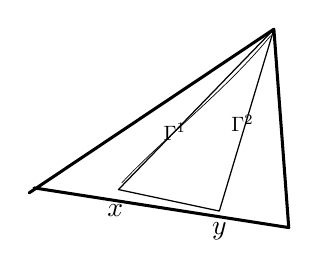
\begin{tikzpicture}[x=.021cm,y=-.021cm,line join=round,line cap=round]
\draw[line width=1.1pt] (0,102)--(148,3)--(157,123)--(3,99);
\draw[line width=.45pt] (148,3)--(54,100)--(115,113)--cycle;
\draw[line width=.25pt] (56,96)..controls (79,71) and (119,40)..(146,7);
\node[below] at (52,103) {$x$};
\node[below] at (115,114) {$y$};
\node[inner sep=0pt,scale=.75] at (88,65) {$\Gamma^{1}$};
\node[inner sep=0pt,scale=.75] at (129,60) {$\Gamma^{2}$};
\end{tikzpicture}}
\end{minipage}\hfill
\begin{minipage}[t]{.67\linewidth}
\small
\[
\left\{\begin{aligned}
\Gamma^{1}_{xy}\cap\Gamma^{2}_{xy}&=\{x,y\}\\
\Gamma^{1}_{x,y}\cup\Gamma^{2}_{x,y}&=\Gamma\\
S'(\Gamma^{1}_{\unsure{x|xx}y})\cup S'(\Gamma^{2}_{xy})&=S(\Gamma)\setminus\{x,y\}\unsure{\cap S(\Gamma|S(\Gamma}
\end{aligned}\right.
\]
\uline{NB} Ce n'est pas le \uline{couple} $(\Gamma^{1}_{xy},\Gamma^{2}_{xy})$ qui est déterminé de façon unique mais l'\uline{ens} $\{\Gamma^{1}_{xy},\Gamma^{2}_{x,y}\}$
\end{minipage}

a) op. de \unsure{rajouter|rajout de} \unsure{sommet|sommets}

b) op. de division d'un polygone (par 2 \unsure{sommets|sommet} distincts) en deux lignes polygonales (op. inverse : recollement de 2 lignes polygonales ayant $=$ extrémités).

\figure{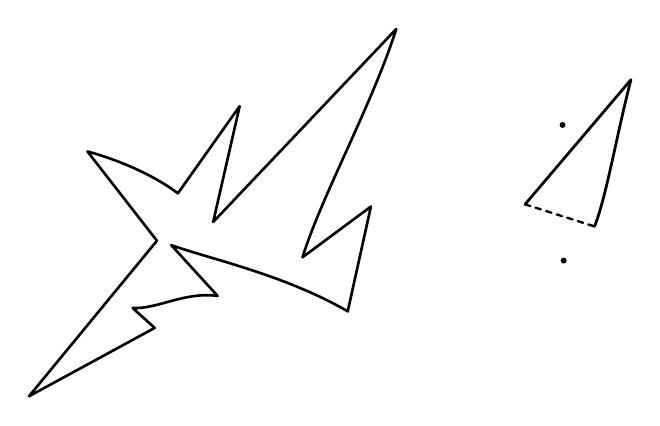
\begin{tikzpicture}[x=.014cm,y=-.014cm,line join=round,line cap=round]
\draw[line width=.95pt] (53,112)..controls (89,122) and (118,137)..(135,150)--(191,71)--(167,176)--(333,1)..controls (311,70) and (265,153)..(248,208)--(310,162)--(289,257)..controls (232,224) and (166,210)..(129,197)--(171,243)..controls (141,239) and (117,255)..(94,254)--(114,272)--(0,334)--(116,193)--cycle;
\begin{scope}[xshift=6.3cm]
\draw[line width=1pt] (0,160)--(96,47)..controls (83,97) and (74,152)..(63,180);
\draw[dash pattern=on 2pt off 2pt,line width=.85pt] (0,160)--(63,180);
\fill (34,88) circle[radius=2.7];
\fill (35,211) circle[radius=2.7];
\end{scope}
\end{tikzpicture}}
% archive sheet number: 21

\scanpage{23}\mspage{II}
$\in S(\Gamma)$ appartient à $\Gamma^{i}_{xy}$ alors $s\in S(\Gamma^{i}_{xy}),\ i=1,2$.
\margin{\tikz[x=.06cm,y=.06cm]{\draw (1,0)--(0,2)--(.2,3)--(-.5,4)--(0,5)--(-.4,6)--(.5,7)--(-.3,7.8)--(-.8,7.2);}}

Si $\Lambda^{1}_{xy}$ et $\Lambda^{2}_{xy}$ sont deux arcs de polygone vérifiant \margin{$\bullet$}$\Lambda^{1}_{xy}\cap\Lambda^{2}_{xy}=\{x,y\}$ on peut obtenir par \unsure{récollement|recollement} selon $\{x,y\}$ un polygone $\Lambda$ de façon évidente.

\margin{\unsure{bien|bis|dir}}%
\margin{$\bullet$}\uline{Definition 1}. On dit \unsure{que'un|qu'un} polygone $\Gamma$ est un $J$-polygone, ou bien que $\Gamma$ est de Jordan si $\Gamma$ vérifie :

a) $\mathbb{R}^{2}-\Gamma=U\cup V$ avec $U$ et $V$ connexes, $U$ relativement compact et \uline{$\overline{V}$ non-compact}, On pose $U=\mathrm{int}\,\Gamma$, $V=\mathrm{ext}\,\Gamma_{\unsure{\bullet|,|x}}$ ;
\margin{$V$\,! non rel. compact}
% slanted

b) Si $D_{x}$ est un disque de centre $x\in\Gamma$ qui ne coupe que les arêtes de $\Gamma$ auxquelles $x$ appartient (deux au plus), alors $D_{x}-D_{x}\cap\Gamma=U'\cup V'$, avec $U'\subset\mathrm{int}\,\Gamma$ et $V'\subset\mathrm{ext}\,\Gamma$ connexes\inserted{(i.e. les 2 comp. conn. de $D_{x}-D_{x}\cap\Gamma$ \deleted{\unsure{appartiennent}} \inserted{sont contenues}, l'une dans $\mathrm{int}\,\Gamma$), l'autre \unsure{ds|dans} $\mathrm{Ext}\,\Gamma$\unsure{)|,}}.
\margin{non \uuline{vides}\,!}
% slanted

\margin{style}%
\uline{Remarque} 2 On voit qu'il suffit qu'un seul disque \deleted{tel} qui ne coupe $\Gamma$ \deleted{ailleurs} que dans les \deleted{\illegible{1}} arêtes auxquelles $x$ appartient vérifie la propriété de b), pour que tout autre \inserted{ayant cette \deleted{\unsure{mê|m}} même propriété} disque \inserted{la} vérifie \inserted{(car \inserted{si $D_{x}\subset D'_{x}$,} $\pi_{0}(D_{x}-D_{x}\cap\Gamma)$ $\longrightarrow$ $\pi_{0}(D'_{x}-\unsure{D'_{\bullet}|D'_{x}}\cap\Gamma)$ est bijectif)}

On pose $R_{\Gamma}=\mathrm{int}\,\Gamma\cup\Gamma$.

\margin{$\cdot$}\uline{Definition} 2. On dit que $s\in S(\Gamma)$ est un \uline{bon sommet} de $\Gamma$ s'il \margin{,}n'est pas colineaire avec les deux sommets $s',s''$ qui sont adjacents à $s$, et si le triangle de sommets $s,s',s''$ ne contient aucun sommet de $\Gamma$ à l'interieur. \inserted{(On \uline{suppose connue} la \uline{notion} de interieur ou de exterieur d'un triangle\unsure{.)|).}}

\margin{vague}%
\inserted{\uline{Déf 3}?}

% The marginal pen strokes flank the two paragraphs on the bottom strip.
\margin{\tikz[x=.1cm,y=.1cm]{\draw (0,0)..controls (.2,1.2) and (1.3,.4)..(1.5,1.4);}}%
\margin{\rule{.35pt}{1em}}%
Si $E$ est une partie de $\mathbb{R}^{2}$ \inserted{et $s,s'\in\mathbb{R}^{2}$,} on dit que $s'$ est $E$-visible de $s$ si le segment \margin{\tikz[x=.1cm,y=.1cm]{\draw (0,0)--(0,1) (0.4,.65)--(1.5,.65)--(1.5,0);}}ouvert $]s,s'[$ est contenu dans $E$ \deleted{$/s,s'\in\mathbb{R}^{2}/$}.

\margin{\rule{.35pt}{1em}}Si $\Gamma$ est un $J$-polygone on dit que $s'$ est visible de $s$ de l'exterieur \inserted{(resp. interieur)} de $\Gamma$ si $s'$ est $\mathrm{ext}\,\Gamma$ (res. $\mathrm{int}\,\Gamma$) - visible de $s$.\margin{\rule{.35pt}{1em}}
% archive sheet number: 22

\scanpage{24}
\figure{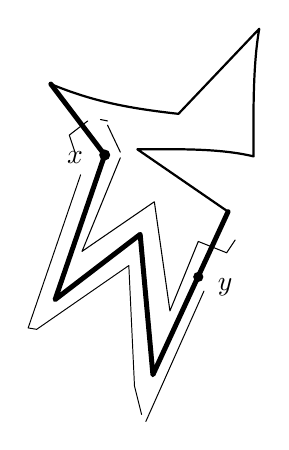
\begin{tikzpicture}[x=.018cm,y=-.018cm,line join=round,line cap=round]
\draw[line width=.8pt] (22,39)..controls (51,51) and (76,56)..(112,60)--(169,0)..controls (164,28) and (165,68)..(165,90)..controls (140,84) and (109,85)..(83,85)--(147,129);
\draw[line width=1.8pt] (22,39)--(60,89)--(25,191)--(85,145)--(94,244)--(147,129);
\draw[line width=.38pt] (48,65)--(35,75)--(39,87) (57,64)--(62,65) (62,68)--(71,87);
\draw[line width=.38pt] (71,91)--(44,157)--(95,122)--(106,199)--(126,150)--(146,158)--(152,149);
\draw[line width=.35pt] (43,103)--(6,211)--(12,212)--(77,167)--(81,252)--(86,272);
\draw[line width=.36pt] (89,277)--(130,185);
\fill (60,89) circle[radius=3.9];
\fill (126,175) circle[radius=3.6];
\node[inner sep=0pt] at (39,91) {$x$};
\node[inner sep=0pt] at (145,182) {$y$};
\end{tikzpicture}}

% The lower strip shows through horizontally reversed. The direction is restored
% here to read the three lines. Two lines carry a stroke through their text.
\margin{\tikz[x=.07cm,y=.07cm]{\draw (0,0)--(.1,-.6) (.15,-1.4)--(.1,-2.8);}}%
\uline{\unsure{Definition|Définition}} 3. Si $\Gamma$ est un polygone et $s,s'\in\mathbb{R}^{2}-\Gamma$ on dit que
\deleted{$s$ est visible de $s'$ ou bien que le couple \inserted{\unsure{de points} $s,s'$} est mutuellement visible si}

\margin{\tikz[x=.07cm,y=.07cm]{\draw (0,0)--(.12,-1) (.1,-1.45)--(-.14,-2.8);}}%
\margin{\tikz[x=.07cm,y=.07cm]{\draw (.15,0)..controls (.35,-.4) and (0,-.8)..(-.1,-1.2) (-.1,-1.5)..controls (0,-1.9) and (.1,-2.25)..(-.1,-2.7);}}%
\[
\deleted{\unsure{[s,s']|]s,s'[}\unsure{-|=}\{s,s'\}\unsure{\subset|\in}\mathbb{R}^{2}-\Gamma.}
\]
% archive sheet number: 23

\scanpage{25}\mspage{III}
\margin{\tikz[x=.08cm,y=.08cm]{\draw (0,0)..controls (1,1.1) and (2.1,1.9)..(1.4,2.8);}}%
\uline{Lemme I}. Soit $\Gamma$ un $J$-polygone et $x,y\in\Gamma$ \inserted{$x\ne y$} ; si $\Gamma^{*}_{xy}$ est l'un de deux arcs de polygone réliant $x$ à $y$, décrit dans la Remarque 1, \margin{!\ \tikz[x=.07cm,y=.07cm]{\draw (0,0)..controls (.4,2) and (1.7,2.4)..(1.5,3.4);}}il \uline{existe un système} fondamental \inserted{$\beta$} de voisinages \deleted{$\unsure{\beta|B}$} \inserted{ouverts} de $\Gamma^{*}_{xy}$ tel que $V\in\beta$ vérifie :
\margin{$\cdot$}
\[
\begin{aligned}
&V\cap\mathrm{int}\,\Gamma\quad\text{et}\quad V\cap\mathrm{ext}\,\Gamma\quad\text{sont connexes (donc}\\
&V-V\cap\Gamma=(V\cap\mathrm{int}\,\Gamma)\cup(V\cap\mathrm{ext}\,\Gamma)\ \text{a deux composantes connexes)}
\end{aligned}
\]

\margin{!}\uline{Demonstration}. gr\uline{âce à l'axiom du c}hoix il suffit de prouver que si $U$ est un voisinage \uline{de $\Gamma$}, \margin{!\\$\Gamma_{xy}$}il existe un voisinage ouvert $V\subset U$ satisfaisant \inserted{à} la condition de l'ennoncé. Pour chaque $z\in\Gamma_{xy}$ on choisit un disque \inserted{ouvert} $D_{z}\subset U$ et satisfaisant b) de la definition 1\unsure{3|,|;} par rapport a $\Gamma$. Il est clair que $\{D_{z}\}_{\inserted{z\in\Gamma_{xy}}}$ est un récouvrement ouvert de l'ensemble compact $\Gamma_{xy}$. Soit donc un sous-récouvrement fini $\{D_{z_{i}}\}^{n}_{i=1}$ de $\Gamma_{xy}$.

Soit $I_{i}$ l'intervalle \inserted{ouvert ou semiouvert de $\Gamma_{xy}$} decoupé par $D_{z_{i}}$, i.e. \inserted{\tikz[baseline=(f.base)]{\node[inner xsep=.12em,inner ysep=.12ex] (f) {$\deleted{\unsure{I|F}}\Gamma_{xy}\cap D_{z_{i}}=I_{i}.$}; \draw[line width=.5pt] ([xshift=-.65em]f.south west)--(f.south west)--(f.north west); \draw[line width=.5pt] ([xshift=.30em,yshift=.35ex]f.north west)--([yshift=.65ex]f.north east)..controls ([xshift=.12em,yshift=.58ex]f.north east) and ([xshift=.15em]f.south east)..([xshift=.23em]f.south east)--([xshift=.45em]f.south east);}} On observe que si $I_{i}\cap I_{j}\ne\phi$ alors $D_{z_{i}}\cap D_{z_{j}}\cap\mathrm{int}\,\Gamma\ne\phi$. Cela permet de montrer que si $z',z''\in\bigcup\limits_{i=1}^{n}D_{z_{i}}\cap\mathrm{int}\,\Gamma$ il existe une suite :

$D_{z_{i_{1}}}\cap\mathrm{int}_{\Gamma},\ \ldotp\;\ldotp\;-\,{-},\ D_{z_{i_{m}}}\cap\mathrm{int}\,\Gamma$ d'ouverts connexes (par le choix de chaque $D_{z}$) tels que $D_{z_{i_{\alpha}}}\cap D_{z_{i_{\alpha+1}}}\cap\mathrm{int}\,\Gamma\ne\phi$ pour $1\le\alpha\le m-1$, et $z'\in D_{z_{i_{1}}}\cap\mathrm{int}_{\Gamma},\ z''\in D_{z_{i_{m}}}\cap\mathrm{int}\,\Gamma$. Ces deux propriétés verifiées par $\bigcup\limits_{i=1}^{n}D_{z_{i}}\cap\mathrm{int}\,\Gamma$ suffisent à prouver la connexité de $\bigcup\limits_{i=1}^{n}D_{z_{i}}\cap\mathrm{int}\,\Gamma$.

\margin{!\ $\cdot$}\deleted{\unsure{Une|Un}} Le même argument prouve (qui\uline{tte à changer $\mathrm{int}\,\Gamma$ par $\mathrm{ext}\,\Gamma$}) que $\bigcup\limits_{i=1}^{n}D_{z_{i}}\cap\mathrm{ext}\,\Gamma$ est connexe. Par conséquent il suffit de prendre $V=\bigcup\limits_{i=1}^{n}D_{z_{i}}$, Cela montre le lemme.

\margin{$\bullet$\quad\uline{?}}On\textsuperscript{\unsure{$*$}} utilise le fait, \uline{sans le dire}, que \deleted{tout couple de} \inserted{deux} points $x,y$ \deleted{\unsure{de|un}} \inserted{d'un} ouvert connexe de $\mathbb{R}^{2}$ peu\deleted{t}\inserted{vent} être reliés par un arc de polygone.
% archive sheet number: 24

\scanpage{26}
% Cancelled block at the foot of the scan, written upside down.
\deleted{Lemme I. Soit $\Gamma$ un $J$-polygone et $x,y\in\Gamma$, si $\Gamma^{1}_{xy}$ est l'un de deux arcs de polygone réliant $x$ à $y$, il existe un système fondamental $\beta$ de voisinages ouverts \inserted{de $\Gamma^{1}_{xy}$}, tel que si $V_{\boxed{\unsure{\Gamma_{xy}|xy}}}\in\beta$ il vérifie}
% archive sheet number: 25

\scanpage{27}\mspage{IV}
2 - \uline{Rappel sur les sous-ensembles convexes de $\mathbb{R}^{2}$}.

\margin{!}\uline{Lemme II}. Si $A$ est une partie \inserted{\uline{finie}} de $\mathbb{R}^{2}$ contenant trois points affinement independants, il existe un polygone et un seul $\Gamma$ tel qu'il n'y ait pas trois sommets consecutifs colineaires \inserted{de $\Gamma$}, et \deleted{de façon} que l'ensemble sous-jacent à $\Gamma$ soit égal a $E(A)-\overset{\circ}{E(A)}$ ($E(A)=$ enveloppe convexe de $A$).

On a aussi $S(\Gamma)\subset A$.

\margin{jargon\\\tikz[x=.12cm,y=.12cm,baseline=0pt]{\draw (0,0)--(.12,-.10)--(.85,3.3);}\quad ?\\$\cdot$}%
% slanted
\uline{Demonstration} (\unsure{Esquisse|Esquissè|Esquissé}) Cela résulte du fait que $E(A)=\tikz[baseline=(q.base)]{\node[inner sep=1pt] (q) {$\cap$};\draw[rotate around={-12:(q.center)}] (q.center) ellipse (.17cm and .35cm);}$ demi espaces fermés correspondants à un ensemble de droites uniquem\uline{ent determinées par} la donnée de $A$, On remarque aussi que $S(\Gamma)=$ \inserted{ens. des} points extremaux de $E(A)$.

\margin{!!!\\partie \unsure{polyédr.l|polyédral|polyédrale} conv.}%
% slanted
\uline{Convention} : Le mot ensemble convexe désigne \uline{pour nous} l'enveloppe convexe d'un ensemble fini de points dans $\mathbb{R}^{2}$. \inserted{Soit $\mathbb{C}$ un \uline{ensemble convexe},} Si l'interieur est non-vide on munit $\partial\mathbb{C}=\mathbb{C}-\overset{\circ}{\mathbb{C}}$ de la structure de polygone décrite dans le lemme II. Il est clair qu'un \uline{ensemble convexe} $\mathbb{C}$ est compact et \inserted{par conséquent} $\partial\mathbb{C}=\mathbb{C}-\overset{\circ}{\mathbb{C}}$ aussi.
\margin{\unsure{intervertir|intervention} \unsure{avec|en} lemme II ! C'est une salade\ldots}

\uline{Lemme III}. Si $s,s'\in\partial\mathbb{C}$, $\overset{\circ}{\mathbb{C}}\ne\phi$, sont deux sommets consecutifs, la droite \deleted{$d$ qui} \inserted{$d$ qu'ils} déterminent partage $\mathbb{R}^{2}$ en deux demi-espaces fermés dont l'un contient $\overset{\circ}{\mathbb{C}}$.

\margin{?\quad ?\\vis\\1}%
\uline{Demonstration} : Cela est trivial quand on exprime $\mathbb{C}$ comme intersection de demi-espaces, si l'on tient compte que $\overset{\circ}{\mathbb{C}}$ est l'intersection des demi espaces ouverts correspondants, et qu'une arète de $\partial\mathbb{C}$ est toujours contenue dans un \uline{tel} demi-espace, c.q.f.d.

\uline{Lemme IV}. Soit $\mathbb{C}$ un \uline{ensemble convexe} à interieur non vide. Si $x\notin\mathbb{C}$ il existe au moins un point $y\in\mathbb{C}-S(\partial\mathbb{C})$ tel que $y$ est $(\mathbb{R}^{2}-C)$-visible de $x$.

\uline{Démonstration} : Choisissons $z\in\overset{\circ}{\mathbb{C}}$ tel que la droite determinée par $x$ et par $z$ \deleted{coupe $\partial\mathbb{C}$} ne contienne aucun sommet de $\partial\mathbb{C}$ (cela est possible car il n'y a qu'un nombre fini de Sommets). Comme $d\cap\mathbb{C}$ est un convexe fermé de $d$ à interieur \inserted{(relatif)} non-vide il est de la forme $d\cap C=[z_{1},z_{2}]$, $z_{1}\ne z_{2}$, il suffit de prendre $y$ \deleted{$\unsure{=y_{1}|=z_{1}}$} egal au point de $[z_{1},z_{2}]$ qui realise le minimum de la distence de $x$ a $[z_{1},z_{2}]$, c.q-f-d.
\margin{!}
% archive sheet number: 26

\scanpage{28}
\figure{%
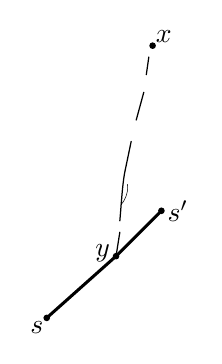
\begin{tikzpicture}[x=0.016cm,y=0.016cm,line cap=round,line join=round]
  \draw[line width=1.1pt] (0,0) -- (55,49) -- (91,85);
  \draw[line width=.45pt]
    (55,49) -- (58,68)
    (58,77) .. controls (59,88) and (60,106) .. (62,116)
    (62,116) -- (67,140)
    (71,157) -- (77,179)
    (79,193) -- (81,207);
  \draw[line width=.2pt] (59,90) .. controls (63,94) and (65,102) .. (64,106);
  \foreach \point in {(0,0),(55,49),(91,85),(84,216)}
    \fill \point circle[radius=1.2pt];
  \node[above right,inner sep=1pt] at (84,216) {$x$};
  \node[left,inner sep=2pt] at (55,51) {$y$};
  \node[below left,inner sep=1pt] at (0,0) {$s$};
  \node[right,inner sep=2pt] at (91,85) {$s'$};
\end{tikzpicture}}
% archive sheet number: 27

\scanpage{29}\mspage{V}
\deleted{$]z,x]\subset\mathbb{R}^{2}-\mathbb{C}$, c.q.f.d.}

% slanted
\margin{\uline{visa}}
\uline{Lemme} V. Soit $\mathbb{C}$ un \uline{ensemble convexe} nonvide de $\mathbb{R}^{2}$ et soit $y\in\mathbb{C}$ tel qu'il existe $s,s'\in\mathbb{C}$ avec $y\in ]s,s'[$. Supposons que $y$ est $(\mathbb{R}^{2}-C)$-visible d'un point $x\notin\mathbb{C}$ qui n'est pas colineaire avec $s$ et $s'$. Alors tout point colineaire avec $s$ et $s'$ est \inserted{$(\mathbb{R}^{2}-\mathbb{C})$-}visible de $x$.

\margin{\uline{NB} $s,s'$ \unsure{appartiennent} \unsure{:|à} une $=$ \unsure{arête|arète} de $C$, et si $D$ est la droite qu'elle détermine $x$ et $C$ sont de part et d'autre de cette droite\ldots}

\uline{Demonstration} : Soit $d$ la droite determinée par $s$ et par $s'$, et appelons $\mathbb{S}_{1}$ et $\mathbb{S}_{2}$ les deux demi-espaces ouverts dans lesquels $\mathbb{R}^{2}$ est partagé par $d$.

Comme $x$ n'est pas colineaire avec $s$ et $s'$, \deleted{\unsure{ou|on}} $x\in S_{1}$ ou bien $x\in S_{2}$.

Supposons que $x\in\mathbb{S}_{1}$ et $z\in d$ et prouvons que $]x,z[\subset\mathbb{R}^{2}-\mathbb{C}$. Si $]x,z[\not\subset\mathbb{R}^{2}\deleted{,}-\mathbb{C}$ il doit exister $w\in ]x,z[\cap\mathbb{C}{}^{\inserted{\subset\mathbb{S}_{1}}}$. Comme $w\in\mathbb{S}_{1}$ aussi, les trois points $s_{\deleted{\unsure{1}}},s_{\deleted{\unsure{2}}}',w$ sont affinement independants.

Considerons donc le triangle $T$ de sommets $s,s',w$ (i.e. l'enveloppe convexe de $\{s',s,w\}$). Comme $[x,\deleted{\unsure{z}}y]\cap ]s,s'[\ne\phi$ on a aussi $[x,y\deleted{\unsure{]}}[\cap T\ne\phi$, mais $T\subset\mathbb{C}$ puisque $\{s,s',w\}\subset\mathbb{C}$ ce qui est un absurd \inserted{puisque on suppose $[x,y[\cap\mathbb{C}=\phi$}, cela prouve donc le lemme.

% A short bent pen stroke in the left margin faces the heading.
\margin{\tikz[baseline]{\draw[line cap=round] (0,0) .. controls (-.02,.16) and (0,.21) .. (.08,.23) -- (.34,.36);}}
\uline{Definition} 3. Un polygone $\Gamma$ est \inserted{dit} convexe \inserted{(par abus de langage !)} si l'ensemble sous-jacent à $\Gamma$ est le bord d'un ensemb\uline{le} \uline{co}nvexe (i.e. $\Gamma=\mathbb{C}-\mathring{\mathbb{C}}$, $\mathbb{C}$ convexe)

\margin{$\bullet$}
On peut maintenant én\deleted{n}oncer le :

\uline{Lemme} VI. Si $\Gamma$ est un polygone convexe alors $\Gamma$ est un J-polygone et tout sommet de $\Gamma$ \deleted{\illegible{1}} qui n'est pas colinéaire avec \deleted{\unsure{s}}les deux sommets adjacents ($=$ consecutifs) est un bon sommet (cf. def.2)
% archive sheet number: 28

\scanpage{30}
% margin note written sideways
\margin{\deleted{alors [les comp. connexes de $\Gamma\cap[s',s'']$ sont des \inserted{côtés et des} segments \unsure{$I_{\alpha}$}, des points \inserted{sommets de \deleted{\unsure{$\Gamma$}}$S$}, et les extrémités des $\unsure{I_{\alpha}}$ et] les \unsure{sg. de} $\unsure{*}$} $S(\Gamma)\cap ]s',s''[\ne\unsure{\psi|\varnothing}$, \deleted{et que, soit $t\in$} alors $\Phi:=S(\Gamma)\cap\unsure{(}T-\{s,s',s''\}\unsure{\}|\!)}\deleted{\unsure{[s',s''])}},\ne\varnothing$, et $t\in\underline{\Phi}$ réalise le maximum de la distance à la droite définie par $s',s''$, alors $]s,t[\subset\operatorname{Int}\Gamma$.}
% margin note written sideways
\margin{\uline{Corollaire} Ou bien $]s',s''[\subset\operatorname{Int}\Gamma$, ou bien $\exists\,t\in S(\Gamma)$, $t\ne\unsure{s}\unsure{\}|{}'}$, tel que $]s,t[\subset\operatorname{Int}\Gamma$.}

\figure{%
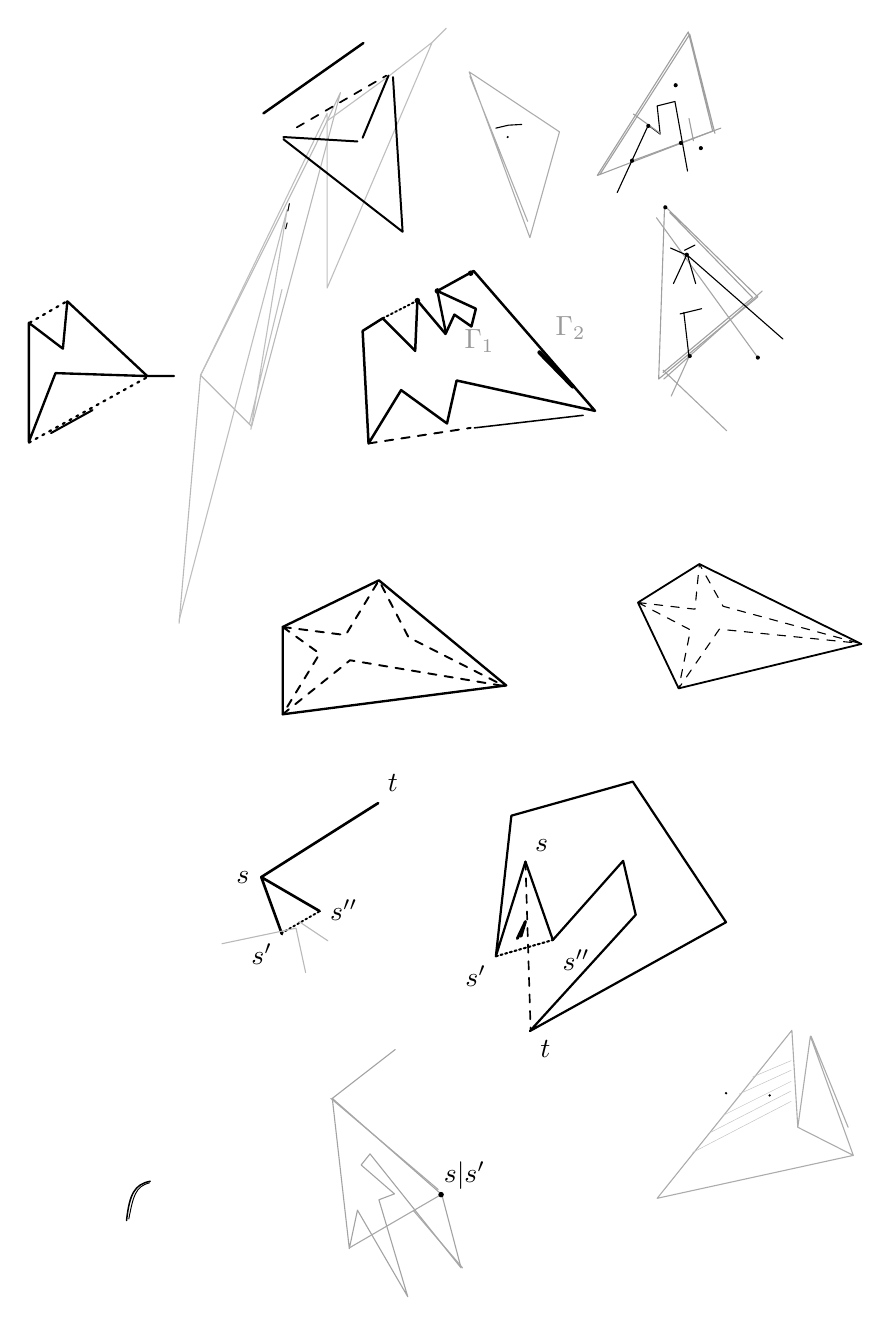
\begin{tikzpicture}[x=.0094cm,y=-.0094cm,line cap=round,line join=round]
% Pencil construction behind the dark reentrant triangle.
  \draw[gray!55] (586,906)--(615,571)--(770,261)--(804,189)--(684,640)--(615,571);
  \draw[gray!50] (586,902)--(732,347)--(683,644)
    (615,571)--(786,217)--(786,453)--(928,121)--(947,102)
    (785,228)--(869,167)--(928,121) (725,455)--(681,637);
  \draw[line width=.37pt] (735,339)--(733,349) (732,365)--(730,373);
  \draw[line width=.9pt] (700,217)--(835,122);
  \draw[line width=.72pt] (727,249)--(827,255) (834,250)--(869,166)
    (875,168)--(888,377)--(727,252);
  \draw[line width=.62pt,dashed] (745,236)--(866,166);
% Small pale triangle to the right.
  \draw[gray!65] (978,161)--(1100,242)--(1060,385)--cycle (979,167)--(1057,363);
  \draw (1014,237)--(1031,233)--(1049,232);
  \fill (1030,249) circle[radius=.43pt];
% Two upper-right pencil triangles and the strokes extended beyond their bases.
  \draw[gray!75] (1151,301)--(1274,107)--(1307,241)--cycle
    (1155,299)--(1276,110)--(1310,244);
  \draw (1178,324)--(1220,233)--(1236,245)--(1232,207)--(1256,201)--(1273,295);
  \draw[gray!75] (1200,218)--(1236,244) (1275,224)--(1281,254) (1196,282)--(1318,237);
  \foreach \p in {(1198,281),(1220,234),(1264,257),(1257,179),(1291,264)} \fill \p circle[radius=.75pt];
  \draw[gray!75] (1242,342)--(1368,465)--(1234,576)--cycle (1249,351)--(1361,466)--(1240,567);
  \draw[gray!70] (1231,358)--(1368,547) (1240,564)--(1326,646)
    (1251,599)--(1275,546) (1241,576)--(1374,457);
  \draw (1402,522)--(1272,408)--(1254,447) (1250,399)--(1273,409)--(1284,447)
    (1268,486)--(1275,546) (1263,488)--(1292,481) (1269,402)--(1283,395);
  \foreach \p in {(1272,408),(1276,545),(1243,344),(1368,547)} \fill \p circle[radius=.75pt];
% Small dark polygon beside the sideways corollary.
  \draw[line width=.85pt] (383,661)--(383,500)--(429,535)--(435,471)--(543,572)
    --(419,568)--cycle (543,572)--(579,572);
  \draw[line width=.8pt,dotted] (384,500)--(436,470) (383,662)--(542,574);
  \draw[line width=.75pt] (413,649)--(469,618);
% Large jagged polygon, including the two pale labels.
  \draw[line width=.9pt] (842,663)--(834,511)--(861,494)--(905,538)--(908,470)
    --(946,515)--(958,489)--(981,505)--(987,481)--(935,457)--(984,430)
    --(1148,619)--(961,578)--(948,636)--(886,591)--cycle;
  \draw[line width=.85pt] (935,457)--(946,511);
  \draw[densely dotted,line width=.7pt] (861,494)--(908,470);
  \draw[dashed,line width=.7pt] (842,663)--(980,642);
  \draw[line width=.55pt] (985,642)--(1132,625);
  \foreach \p in {(908,470),(935,457),(980,433)} \fill \p circle[radius=1pt];
  \draw[line width=1.55pt] (1073,540)--(1118,586);
  \node[gray!80] at (992,525) {$\Gamma_1$};
  \node[gray!80] at (1115,507) {$\Gamma_2$};
% Pair of quadrilaterals with broken interior paths.
  \draw[line width=.85pt] (726,911)--(856,848)--(1028,990)--(726,1029)--cycle;
  \draw[line width=.7pt,dashed] (726,911)--(811,922)--(856,848)--(896,925)--(1026,991)
    (726,911)--(776,947)--(726,1029)--(817,956)--(1026,991);
  \draw[line width=.65pt] (1206,878)--(1289,826)--(1508,934)--(1261,994)--cycle;
  \draw[dashed] (1206,878)--(1283,887)--(1289,826)--(1321,883)--(1505,933)
    (1206,878)--(1277,915)--(1261,994)--(1316,914)--(1505,933);
% Four-point sketch and larger labelled polygon.
  \draw[line width=.95pt] (855,1149)--(697,1249)--(725,1326) (697,1249)--(776,1295);
  \draw[densely dotted,line width=.68pt] (724,1325)--(778,1294);
  \draw[gray!55] (644,1339)--(744,1318)--(757,1378) (748,1309)--(787,1335);
  \node[left] at (694,1249) {$s$};
  \node[below left] at (725,1326) {$s'$};
  \node[right] at (777,1293) {$s''$};
  \node[above right] at (855,1147) {$t$};
  \draw[line width=.8pt] (1014,1356)--(1035,1166)--(1199,1120)--(1325,1310)
    --(1060,1457)--(1203,1300)--(1186,1227)--(1091,1334)--(1054,1228)--cycle;
  \draw[densely dotted,line width=.75pt] (1014,1356)--(1091,1334);
  \draw[dashed,line width=.6pt] (1054,1228)--(1061,1456);
  \draw[line width=1.05pt] (1043,1332)--(1054,1309)--(1048,1329);
  \node[above right] at (1054,1228) {$s$};
  \node[below left] at (1014,1356) {$s'$};
  \node[below right] at (1091,1334) {$s''$};
  \node[below right] at (1061,1456) {$t$};
% Isolated curved pen mark below the sideways corollary.
  \draw[line width=.55pt] (515,1713).. controls (519,1677) and (526,1664)..(547,1660);
  \draw[line width=.35pt] (518,1711).. controls (524,1680) and (527,1667)..(546,1662);
% Lowest pencil studies, with crossed zigzags, dots, and hatching.
  \draw[gray!72] (878,1482)--(793,1548)--(816,1751)--(827,1699)--(895,1816)
    --(856,1685)--(877,1677)--(832,1638)--(844,1623)--(967,1777)
    --(941,1678)--(793,1548);
  \draw[gray!68] (816,1750)--(940,1678) (903,1700)--(969,1777) (791,1548)--(936,1671);
  \fill (940,1678) circle[radius=1pt];
  \node[above right,inner sep=.8pt] at (940,1675) {$\unsure{s|s'}$};
  \draw[gray!65] (1232,1683)--(1414,1456)--(1422,1587)--(1439,1464)--(1497,1625)--cycle
    (1422,1587)--(1497,1625) (1440,1464)--(1490,1587);
  \foreach \x/\y/\v in {1280/1621/1552,1302/1595/1538,1321/1571/1525,1343/1542/1510,1361/1519/1497}
    \draw[gray!45,line width=.19pt] (\x,\y)--(1413,\v);
  \foreach \p in {(1325,1541),(1384,1544)} \fill \p circle[radius=.47pt];
\end{tikzpicture}}
% crop-candidate: scan 30

\uline{Lemme} Soit $\Gamma$ un \deleted{\unsure{J}}polygône \deleted{à $n\ge4$ côtés} \inserted{à $n$ côtés $(n\ge3)$}. Alors $\exists\,s\in S(\Gamma)$ \inserted{``non plat''} tel que $\forall\,D_s$ de centre $s$, \deleted{l'un des} satisfaisant la cond. b) de Déf 1, le secteur angulaire de $D$ découpé par $\Gamma$ (i.e. par $[s,s']\cup(s,s'']$ où $s',s''$ sont les $2$ sommets adjacents) qui est d'angle $>\pi$ soit \uline{extérieur} à $\Gamma$. Si $\Gamma$ est un J-polygône, et $n\ge4$, alors
\[
\begin{aligned}
&\text{(i) Si }\ \Gamma\cap\deleted{\unsure{\operatorname{Int}}}\overset{\deleted{\unsure{\circ}}}{T}=[s,s']\cup[s,s''],\quad ]s',s''[\ \deleted{\unsure{\text{est}}}\subset\operatorname{Int}\Gamma\ \text{\deleted{\unsure{et si}}}\\
&\text{(ii) Si }\ \Gamma\cap T\ne[s',s']\cup[s,s'']\quad
\deleted{\text{et }\Gamma\cap\mathring{T}=\varnothing,\ \unsure{\text{que}}\ \unsure{\Gamma\cap T}\ ]s',s''[\subset\operatorname{Int}}
\end{aligned}
\]
% archive sheet number: 29

\scanpage{31}\mspage{VI}
\uline{Demonstration} : Supposons $\Gamma=\partial\mathbb{C}$, avec $\mathbb{C}$ convexe et compact.

On prend $\operatorname{int}\Gamma=\mathring{\mathbb{C}}$ et $\operatorname{ext}\Gamma=\mathbb{R}^{2}-\mathbb{C}$. Il est clair que $\operatorname{int}\Gamma=\mathring{\mathbb{C}}$ est convexe puisque l'interieur d'un ensemble convexe est convexe.

Pour montrer que $\mathbb{R}^{2}-\mathbb{C}$ est connexe on choisit \inserted{le bord $\partial T$ d'}un triangle $T$ (qui vérifie la propiété d'être un J-polygone par des raisons elementaires) et on montre que $(\partial T\cup\operatorname{int}\partial T)-\mathbb{C}$ est connexe. Soit $x\in\partial T\cup\operatorname{int}\partial T$ \deleted{$x\notin\mathbb{C}$,} $(=R_{\partial T})$ \inserted{et $x\notin\mathbb{C}$} et soit $d$ une droite qui passe par $x$. Alors $d\cap\mathbb{C}=\phi$ ou bien $d\cap\mathbb{C}=[z_1,z_2]$\inserted{ avec $z_1,z_2\in\mathbb{C}$}, Dans le premier cas on voit que $x$ peut être \unsure{reliér|relié} à un point de $\partial T$ puisque $d\cap\partial T\ne\phi$.

Si $d\cap\mathbb{C}=[z_1,z_2]$ soit $z_1$ le point \inserted{de $\mathbb{C}$} le plus proche à $x$ sur $d$, alors la demi-droite fermée d'origine \deleted{$\unsure{z|x}$}$z_1$ qui contient $x$ coupe aussi $\partial T$. Donc dans tous le cas $x$ peut être relié a $\partial T$ et cela montre la connexité de $\overset{\inserted{\substack{T\\\Vert}}}{(\partial T\cup\operatorname{int}\partial T)}-\mathbb{C}$, comme $(\mathbb{R}^{2}-T)\cup\partial T$ est connexe \inserted{(fermeture d'un connexe)} \margin{\tikz[x=.08cm,y=-.08cm]{\foreach \x/\y in {1/0,1/1.1,.8/1.5,.75/2.1,.6/2.3,0/2.8,.4/3.4}\fill (\x,\y) circle[radius=.35pt];}}on a montré la propiété \deleted{\unsure{b}}a) de la definition 2. La propiété b) est une application \inserted{simple} du lemme .

\margin{$\bullet$}
L'affirmation qui reste est trivial par definition de convexe, \unsure{\(\blacksquare\)|\deleted{\illegible{1}}} c.q.f.d. .

\margin{$\bullet$}
Si $\Gamma$ est un polygone de $\mathbb{R}^{2}$ on considĕre son enveloppe convexe, $E(\Gamma)$.

\margin{réf \unsure{juste.}}
Il est \uline{clair} que $E(\Gamma)$ vérifie :
\[
\begin{aligned}
\text{a)}\quad & E(\Gamma)=E(S(\Gamma))\quad;\\
\text{b)}\quad & \underset{\inserted{S(\partial(\unsure{E(\Gamma|E\Gamma}))}}{S(\partial(\Gamma))}\subset S(\Gamma)\quad.
\end{aligned}
\]

On veut étudier le lien entre $\Gamma$ et son enveloppe convexe.
% archive sheet number: 30

\scanpage{32}
\uline{Lemme} \unsure{Soient|Soit} $\Gamma,\Gamma'$ deux polygônes \deleted{\unsure{tels que} $\Gamma=$} \inserted{distinct,} alors $\Gamma\not\subset\Gamma'$, $\Gamma'\not\subset\Gamma$, et $\Gamma\cap\Gamma'$ est une réunion finie d'arcs disjoints de $\Gamma$ (ou de $\Gamma'$), éventuellement réduits à un point.
\figure{%
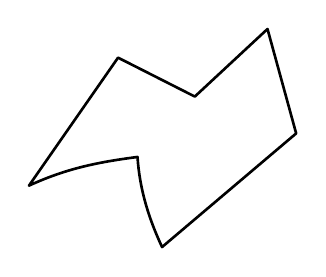
\begin{tikzpicture}[x=.013cm,y=-.013cm,line cap=round,line join=round]
  \draw[line width=.95pt] (274,1178)--(361,1053)--(436,1091)--(507,1025)
    --(535,1127)--(404,1238).. controls (390,1208) and (382,1180) ..(380,1150)
    .. controls (342,1155) and (311,1161) ..(274,1178)--cycle;
\end{tikzpicture}}
Si $\Gamma'=\partial E(\Gamma)$, où $\Gamma$ est un polygône (non convexe puisque $\Gamma'\ne\Gamma$), alors l'\deleted{\unsure{ens}} \inserted{$\Phi$ des} extrémités des arcs polygonaux composantes connexes de $\Gamma\cap\Gamma'$ \deleted{sont des sommets de $\Gamma$} \inserted{est $\subset S(\Gamma)$} alors toute \deleted{telle} $s\in\Phi$, $\exists\,\deleted{\unsure{E}}t\in\Phi$, $t\ne s$, telle que $]s,t[\subset\Gamma'\deleted{\unsure{\operatorname{Ext}}}\cap\complement\Gamma$ et alors $]s,t[\subset\operatorname{Ext}\Gamma$.

% slanted
\margin{\uline{NB} $t$ est unique, sauf si $s$ point isolé de $\Gamma\cap\Gamma'$, auquel cas il existe \unsure{exactmt|exactem} deux tels $t$.}

\uline{Cor} Si $\Gamma$ polygône non convexe, $\exists\,s,s'$ sommets distinct de $\Gamma$, tel que $s$ \deleted{et $s'$, \unsure{visib} de $s$} $]s,s'[\subset\operatorname{Ext}\Gamma\cap\partial E(C)$

[\uline{NB} $\operatorname{Ext}(\Gamma)$ est défini pour tt polygône, pas néc. un 'J-polygône\unsure{.-|..} ]
% archive sheet number: 31

\scanpage{33}\mspage{VII}
\uline{Lemme} VII : Si $\Gamma$ est un J-polygone on a $\operatorname{ext}\partial E(\Gamma)\subset\operatorname{ext}\Gamma$.

\uline{Démonstration} : Comme $E(\Gamma)$ est un ensemble convexe $\operatorname{ext}\partial E(\Gamma)=\mathbb{R}^{2}-E(\Gamma)$ (d'aprés la preuve du lemme VI) donc $\operatorname{ext}\partial E(\Gamma)\cap\Gamma=\phi$ puisque $\Gamma\subset E(\Gamma)$.

Il est clair que $\operatorname{ext}\Gamma\cap\operatorname{ext}\partial E(\Gamma)\ne\phi$ (par exemple en prenant un triangle qui contient $R_{\Gamma}$ et $R_{\partial E(\Gamma)}$ à l'interieur on voit que l'exterieur est \unsure{comun|commun} à \deleted{\unsure{à|la}} $\operatorname{ext}\Gamma$ et a $\operatorname{ext}\partial E(\Gamma)$). Donc $\operatorname{ext}\partial E(\Gamma)\subset\operatorname{ext}\Gamma$ puisque $\operatorname{ext}\partial E(\Gamma)$ est connexe \inserted{et $\mathbb{R}^{2}-\Gamma=\operatorname{int}\Gamma\cup\operatorname{ext}\Gamma$.} cela prouve le lemme.

% slanted
\margin{\unsure{inutil|inutile}}
\uline{Lemme VII} : Si $\Gamma$ est un \inserted{(}J-\inserted{)}polygone non-convexe il existe $s,s'\in\mathbb{S}(\Gamma)$ tel que \deleted{\unsure{si}} $s'$ est visible de $s$ de l'exterieur de $\Gamma$.

\uline{Demonstration} : On sait que $\partial E(\Gamma)\cap\Gamma\ne\phi$ (puisque $\deleted{\unsure{\exists}}\partial E(\Gamma)\cap\Gamma\supset\mathbb{S}(\partial E(\Gamma))$) on veut montrer \inserted{que} $\partial E(\Gamma)\not\subset\Gamma$. Si $\partial E(\Gamma)\subset\Gamma$ alors \inserted{on prouve facilement que} $\partial E(\Gamma)$ est un sous-ensemble ouvert de $\Gamma$ et en plus fermé puisqu'il est compact donc $\partial E(\Gamma)=\Gamma$ en raison de la conexité de $\Gamma$, ce qui contredit le fait que $\Gamma$ est non-convexe.

% margin note written sideways
\margin{\deleted{\unsure{Compl.|Conclure|Concl.} \unsure{que} $\partial E(\Gamma)\subset\Gamma\ \Rightarrow\ \underset{\substack{\Vert\\ E(\Gamma)}}{E(\partial E(\Gamma))}\subset$ \unsure{bref}}}
Soit $\alpha$\inserted{$=[s,s']$} une arête de $\partial E(\Gamma)$ telleque $\alpha\not\subset\Gamma$. Si $]s,s'[\subset\mathbb{R}^{2}-\Gamma$ cela prouve le lemme puisque $s,s'\in\mathbb{S}(\Gamma)$.

Si $s$ est un point isolé de $\alpha\cap\Gamma$ Soit $t$ le point de $(\Gamma-s)\cap\alpha$ qui réalise la distance de $s$ a l'ensemble compact $\alpha\cap(\Gamma-s)=\alpha\cap\Gamma-\underbrace{\{s\}}_{\inserted{\text{ouvert dans }\alpha\cap\Gamma}}$. Il est clair par le choix de $t$ que $]s,t[\subset\mathbb{R}^{2}-\Gamma$. Prouvons que $t\in\mathbb{S}(\Gamma)$. Si $t\notin\mathbb{S}(\Gamma)$ il existe $\alpha'\in A(\Gamma)$ tel que $t\in$ au segment ouvert correspondant $=\mathring{\alpha}'$, mais alors comme $t\in\mathring{\alpha}'\cap\mathring{\alpha}$ on doit pouvoir trouver un ouvert $\subset\mathring{\alpha}'\cap\mathring{\alpha}$ \inserted{auquel $t$ appartient} cela contredit le choix de $t$, puisque $\mathring{\alpha}'\cap\mathring{\alpha}\subset\alpha\cap\Gamma$. Si $s$ n'est pas isolé on peut trouver une arête $[s,t_1]\in A.(\Gamma)$ telle que $[s,t_1]\subset\alpha$. Si $t_1$ est isolé on réfait l'argument ci-dessus, dans le cas contraire on considère $[t_1,t_2]$-{}-etc. jusqu'à trouver $t$ isolé dans $[s,s']$.

Montrons maintenant que si $s,s'\in S(\Gamma)$ et $]s,s'[\subset\mathbb{R}^{2}-\Gamma$ si $[s,s']\subset\alpha\subset\partial E[\Gamma]$ $]s,s'[\subset\operatorname{ext}\Gamma$.
% archive sheet number: 32

\scanpage{34}\mspage{VIII}
Comme $]s,s'[\subset\mathbb{R}^{2}-\Gamma$ est connexe on a $]s,s'[\subset\operatorname{int}\Gamma$ ou bien $]s,s'[\subset\operatorname{ext}\Gamma$.

Si $t^{\deleted{\unsure{*|'}}}\in ]s,s'[$ alors $t\in\alpha\subset\partial E(\Gamma)$ \inserted{et \deleted{\unsure{donc}} $t\in\mathbb{R}^{2}-\Gamma$,} Comme $\partial E(\Gamma)$ est un polygone convexe il vérifie la condition b) de la definition 1 (cf. lemme VI), on peut donc choisir $D_t\subset\mathbb{R}^{2}-\Gamma$ satisfaisant b). Mais $D_t\cap\operatorname{ext}\partial E(\Gamma)\ne\phi$ \inserted{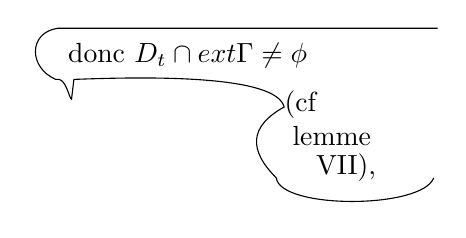
\begin{tikzpicture}[x=1cm,y=1cm,baseline=(line.base)]
\node[anchor=west,inner sep=0pt] (line) at (0,0) {donc $D_t\cap\operatorname{ext}\Gamma\ne\phi$};
\node[anchor=west,inner sep=0pt] at (2.75,-.62) {(cf};
\node[anchor=west,inner sep=0pt] at (2.85,-1.02) {lemme};
\node[anchor=west,inner sep=0pt] at (3.15,-1.42) {VII),};
\draw (4.7,.35)--(-.12,.35) .. controls (-.5,.3) and (-.5,-.15) .. (-.15,-.3)
 .. controls (-.02,-.26) and (.02,-.55) .. (.05,-.55)
 --(.08,-.3) .. controls (1.1,-.26) and (2.65,-.25) .. (2.75,-.65)
 .. controls (2.3,-.9) and (2.3,-1.2) .. (2.65,-1.55)
 .. controls (2.7,-1.95) and (4.5,-1.95) .. (4.65,-1.55);
\end{tikzpicture}} avec le fait que $D_t$ est connexe entraîne $D_t\subset\operatorname{ext}\deleted{\partial E(}\Gamma\deleted{)}$, donc $t\in\operatorname{ext}\deleted{\partial E(}\Gamma\deleted{)}$ ce qui prouve \inserted{que} $]s,s'[\deleted{\subset}\deleted{\mathbb{R}^{2}-E(\Gamma)=}\deleted{\operatorname{ext}\partial E(\Gamma)}\subset\operatorname{ext}\Gamma$, \deleted{en vertu du lemme VII}, c.q.f.d.

Si $\Gamma$ est un J-polygone et $s\in S(\Gamma)$, soit $D_s$ un disque de centre $s$ satisfaisant à b) de la def.\deleted{\unsure{2}}1, puisque $s$ appartient a deux arêtes de $\Gamma$ on a que $\Gamma\unsure{\Vert|\cap}D_s$ determine deux secteurs angulaires dont l'interieur de l'un est contenu dans $\operatorname{int}\Gamma$ (secteur interieur) et l'interieur de l'autre dans $\operatorname{ext}\Gamma$ (secteur exterieur).

\margin{$\unsure{\cdot|\bullet}$}
On a \deleted{donc} \inserted{alors} l'analogue suivant de la positivité de la courbure des courbes \inserted{de $\mathbb{R}^{2}$} convexes :

\uline{Lemme} IX : Si $\Gamma$ est un polygone convexe et $s\in\mathbb{S}(\Gamma)$ alors pour tout disque $D_s$ de centre $s$ qui satisfait b) de la def. 2 l'angle $\alpha$ qui ``sous tend'' le secteur circulaire interieur \unsure{vérifie|vérifié} $\alpha\le\pi$.

\uline{Demonstration} : Comme le secteur ang. interieur $=\overbrace{D_s}^{\inserted{\text{convexe}}}\cap\overbrace{\operatorname{int}\Gamma}^{\inserted{\text{convexe}}}$, on voit qu'il est convexe, mais un secteur angulaire est convexe si et seulement si on angle $\alpha$ vérifie $\alpha\le\pi$, c.q.f.d. .

\deleted{\unsure{Lemme} \illegible{3}}

\uline{Lemme X} : Si $\Gamma$ est un \deleted{J-}polygone il existe au moins trois sommets tels que pour tout disque $D_s$ qui satisfait b) \deleted{\illegible{1}}. de la def. 2 et de centre un de ces trois sommets l'angle du secteur angulaire interieur est inferieur à $\pi$.

\uline{Demonstration} : Soit $s\in\mathbb{S}(\partial E(\Gamma))\subset S(\Gamma)$ et soient $s',s''$ les deux sommets de $\partial E(\Gamma)$ qui sont consecutifs à $s$. Le lemme II nous dit que $s,s',s''$ ne sont pas colineaires.
% archive sheet number: 33
